\documentclass[12pt,a4paper]{book}
\usepackage[utf8]{inputenc}
\usepackage[spanish]{babel}
\usepackage{amsmath}
\usepackage{amsfonts}
\usepackage{amssymb}
\usepackage{latexsym}
\usepackage{makeidx}
\usepackage{amssymb}
\usepackage{graphicx}
\usepackage{graphics}
\usepackage{lmodern}
\usepackage{hyperref}
\usepackage{subcaption}
\usepackage{pgfplots}
\usepackage{dsfont}
\usepackage{multicol}
\usepackage{xcolor}
\usepackage{booktabs}
\usepackage{float}
\usepackage{subcaption}
\pgfplotsset{width=10cm,compat=1.9}
\usepgfplotslibrary{external}


\setlength{\parindent}{15px}
\usepackage[left=2cm,right=2cm,top=4cm,bottom=2cm]{geometry}

\author{Daniel Vázquez Lago}
\title{Apuntes Mecánica Clásica II}


\newcommand{\parentesis}[1]{\left( #1  \right)}
\newcommand{\parciales}[2]{\frac{\partial #1}{\partial #2}}
\newcommand{\pparciales}[2]{\parentesis{\parciales{#1}{#2}}}
\newcommand{\ccorchetes}[1]{\left[ #1  \right]}
\newcommand{\D}{\mathrm{d}}
\newcommand{\derivadas}[2]{\frac{\D #1}{\D #2}}
\newcommand{\sech}{\mathrm{sech} \ }
\newcommand{\csch}{\mathrm{csch} \ }
\newcommand{\cotanh}{\mathrm{cotanh}}
\newcommand{\cotan}{\ \mathrm{cotan}}
\newcommand{\Det}{\ \mathrm{det}}
\newcommand{\Res}{\mathrm{Res}}
\newcommand{\Arg}{\mathrm{arg}}
\newcommand{\vecu}{\vec{u}}
\newcommand{\vecv}{\vec{v}}
\newcommand{\tquad}{\quad \quad \quad}
\newcommand{\intx}{\int_{x_1}^{x_2}}


\newcommand{\rn}{\mathbf{r}}
\newcommand{\Rn}{\mathbf{R}}
\newcommand{\Ln}{\mathbf{L}}
\newcommand{\Pn}{\mathbf{P}}

\newtheorem{theorem}{Teorema}[section]
\newtheorem{corollary}{Corolario}[theorem]
\newtheorem{lemma}{Lema}[section]
\newtheorem{ejemplo}{Ejemplo}[section]


\begin{document}

\maketitle

\newpage

\tableofcontents

\newpage

\chapter{Formulación Lagrangiana}
\section{Introducción}

En este tema vamos a estudiar una nueva forma de obtener las ecuaciones del movimiento. Como sabemos para ir de un punto A a un punto B podemos tomar diferentes caminos (infinitos caminos). En este punto el problema de la dinámica se reduce a cómo singularizar uno de ellos, de tal forma que hallemos la trayectoria que sigue realmente el objeto estudiado. \\

En 1834 Hamilton formula un principio que nos da la manera de elegir entre todas las posibles trayectorias del espacio de configuración compatibles con las ligaduras que puede seguir un sistema dinámico al evolucionar de un estado a otro en un tiempo determinado. Este principio nos dice que la trayectoria seguida es aquella que hace mínima la acción. \\

Es un principio sencillo y muy bonito. En otras ramas de la física se usan principios parecidos para describir el comportamiento de algunos fenómenos. Ejemplos pueden ser el cálculo de geodésicas o el principio de Frenet de la óptica, que nos dice que los rayos de luz siguen el camino que hace que el tiempo invertido sea el menor posible (entre dos puntos). \\

Sin embargo para poder avanzar al tratar este principio tenemos que definir primero que es la acción, y para ello debemos ver que es un \textit{funcional}.

\subsection{Ecuaciones de Euler-Lagrange}

Supongamos una curva $y=y(x)$ continua y diferenciable. Definimos como \textbf{funcional} a la integral curvilínea de una función $f(y',y,x)$ (que solo depende de $x$ ya que $y(x),y'(x)$) entre dos puntos $x_1$ y $x_2$. Dicho de otra forma, el funcional $J$ se define como:

\begin{equation}
J = \int_{x_1}^{x_2} f(y',y,x) \D x 
\end{equation}

Ahora tenemos que aplicarle algún tipo de condición a nuestra función. Supongamos que nuestra función $y$ verifica que para los puntos $x_1$ y $x_2$:

\begin{equation}
y(x_1) = y_1 \tquad y(x_2) = y_2
\end{equation}

Según el principio de Hamilton el funcional acción debe de minimizarse, por lo vamos a buscar para que $y(x)$ se minimiza esta acción. Entonces introduciremos una familia de curvas parametrizadas en función de $\alpha$. Asignamos arbitrariamente que $y(x)$ cuando $\alpha=0$ es la que extremiza la función, escribiendo nuestra función como:

\begin{equation}
y (x,\alpha) = y(x) + \alpha \eta (x)
\end{equation}

si escogemos una función arbitraria $\eta(x)$ tal que:

\begin{equation}
\eta (x_1) = 0; \tquad \eta(x_2) = 0
\end{equation}

en este caso se verificará completamente que la función $y(x,\alpha)$ pase por los puntos $y_1$ e $y_2$ para cualquier $\alpha$, por lo que tenemos una familia de curvas que pasa por estos dos puntos. \\

Nuestro funcional $J$ ahora dependerá de $\alpha$:

\begin{equation}
J(\alpha) = \int_{x_1}^{x_2} f(y'(\alpha,x),y(\alpha,x),x) \D x 
\end{equation}

Desarrollemos en serie de taylor a $J$ en función de la única variable de la que depende, centrándola en $\alpha = 0$, de tal forma que:

\begin{equation}
J(\alpha) = J(\alpha = 0) +  \left. \dfrac{\D J}{\D \alpha} \right|_{\alpha = 0} \cdot \alpha + \cdots
\end{equation}

de tal modo que podamos considerar un desplazamiento virtual

\begin{equation}
\delta J = J (\alpha) - J(\alpha = 0) \simeq \left. \dfrac{\D J}{\D \alpha} \right|_{\alpha = 0} \cdot \alpha
\end{equation}

donde hemos supuesto que los términos con las potencias superiores son despreciables. El mismo desplazamiento virtual de $y$ será:

\begin{equation}
\delta y(x,\alpha) = y(x,\alpha) - y(x,0) = \left. \dfrac{\D y}{\D \alpha} \right|_{\alpha = 0} \cdot \alpha = \alpha \cdot \eta (x)
\end{equation}

Para que la condición de extremo se verifique:

$$ \delta J = 0 \Leftrightarrow \left. \dfrac{\D J}{\D \alpha} \right|_{\alpha = 0} = 0 $$

y si usamos la regla de la cadena:

$$ \dfrac{\D J}{\D \alpha}= \dfrac{\D}{\D \alpha} \int_{x_1}^{x_2} f(...) \D x = \int_{x_1}^{x_2} \dfrac{\D f}{\D \alpha} \D x  = \int_{x_1}^{x_2} \parentesis{\parciales{f}{y}\parciales{y}{\alpha} + \parciales{f}{y'}\parciales{y'}{\alpha}} \D x $$

y fijándonos que:

\begin{align*}
\intx \D x \parentesis{\parciales{f}{y'}\parciales{y'}{\alpha}} & = \intx \D x \parentesis{\parciales{f}{y'} \parciales{}{\alpha} \parentesis{ \dfrac{\D y }{\D x} }} = \intx \D x \parentesis{\parciales{f}{y'} \dfrac{\D}{\D x} \parentesis{ \parciales{y }{\alpha} }} \\
     & = \intx \D x \parentesis{\dfrac{\D}{\D x} \parentesis{\parciales{f}{y'} \parciales{y}{\alpha}}} - \intx \D x \parentesis{\parciales{y}{\alpha} \dfrac{\D}{\D x} \parentesis{\parciales{f}{y'}}}   \\
     & =  \ccorchetes{\parciales{f}{y'} \parciales{y}{\alpha}}_{x_1}^{x_2} - \intx \D x \parentesis{\parciales{y}{\alpha} \dfrac{\D}{\D x} \parentesis{\parciales{f}{y'}}}
\end{align*}
 
Dado que 

$$ \parciales{y}{\alpha} = \eta (x); \tquad \eta(x_1)=\eta (x_2) = 0$$

se tiene que:

$$ \ccorchetes{\parciales{f}{y'} \parciales{y}{\alpha}}_{x_1}^{x_2} = 0 $$

y por lo tanto:

\begin{equation}
\dfrac{\D J}{\D \alpha} = \intx  \parentesis{\parciales{y}{\alpha}} \parentesis{\parciales{f}{\alpha}-\dfrac{\D}{\D x}\parciales{f}{y'}} \D x = \intx  \eta (x) \parentesis{\parciales{f}{\alpha}-\dfrac{\D}{\D x}\parciales{f}{y'}} \D x
\end{equation}

Por lo que se verificará la condición de extremo del funcional si:

\begin{equation}
\parciales{f}{y} - \dfrac{\D}{\D x} \parentesis{\parciales{f}{y'}} = 0
\end{equation}

que es la \textbf{ecuación de euler} para la curva $y(x)$. Si nuestro funcional $J$ dependiera de $n$ curvas $y_j(x)$, la condición de extremo del funcional serían las \textit{n ecuaciones de Euler}:

\begin{equation}
\dfrac{\D}{\D x} \parentesis{\parciales{f}{y_j'}} - \parciales{f}{y_j} = 0
\label{Ec:1.1.012}
\end{equation}

\section{Principio de Hamilton}

Como ya hemos mencionado el problema de la dinámica se reduce a hallar la curva que minimiza la acción, que es lo que enunciamos como \textbf{principio de Hamilton}. Para sistemas conservativos este expresa que: ``\textit{el movimiento del sistema entre dos tiempos $t_1$ y $t_2$ es aquel que verifica la condición de extremo del funcional de acción S definido como $S = \int_{t_1}^{t_2} L \D t $ donde $L=T-V$ y la llamamos \textbf{lagrangiana}}''. De manera rigurosa el funcional acción:

\begin{equation}
S = \int_{t_1}^{t_2} L(q_i,\dot{q}_i,t) \D t
\end{equation}

Y como hemos deducido antes las ecuaciones que extremizan un funcional cualquiera son las ecuaciones de euler presentadas en el punto anterior, que se han deducido usando lo que conocemos por \textit{principio variacional} ($\delta S$), y la particularización de las ecuaciones de euler para el caso dinámico llevan a las \textit{ecuaciones de Euler-Lagrange}. \\

\subsection{Sistemas con ligaduras}

Comenzamos para el caso de un sistema con dos coordenadas generalizadas ($x,y$), para luego ampliar el generalizara a un caso con $n$ coordenadas. Existen dos formas de solucionar un problema dinámico si nuestras ligaduras son holónomas (si son holónomas son del tipo $f(x,y) = 0$):

\begin{itemize}
\item Eliminamos una de las coordenadas generalizadas, dejar una de ellas como única variable independiente y grado de libertad, para luego calcular la ecuación del movimiento de esta.

\item Mantener las dos coordenadas y usar la ecuación de la ligadura posteriormente. Este método se conoce como el \textit{método de los multiplicadores de Lagrange} y aunque es mas tedioso nos permite calcular las fuerzas de ligadura.
\end{itemize} 

Consideremos pues el funcional de acción S, si aplicamos el principio variacional:

\begin{equation}
\delta S = \int \parentesis{\parciales{L}{x} - \dfrac{\D}{\D t} \parentesis{\parciales{L}{\dot{x}}}} \delta x \D t + \int \parentesis{\parciales{L}{y} - \dfrac{\D}{\D t} \parentesis{\parciales{L}{\dot{y}}}} \delta y \D t = 0 \label{Ec:1.2.1-013}
\end{equation}

Si ambas coordenadas fueran independientes cada integral tendría que anularse por separado, y por lo tanto obtendríamos dos ecuaciones del movimiento. Sin embargo como tenemos $f(x,y)=0$ los desplazamientos no son independientes, ya que:

\begin{equation}
\delta f = \parciales{f}{x} \delta x + \parciales{f}{y} \delta y = 0
\end{equation}

donde definimos $a_x$ como la parcial de $f$ respecto a $x$ y $a_y$ respecto a $y$. Si multiplicamos dicha ecuación por la función arbitraria $\lambda (t)$ que llamaremos \textit{multiplicador indeterminado de lagrange} obtenemos que:

$$ \lambda (t) \delta f = (a_x \lambda (t)) \delta x + (a_y \lambda (t)) \delta y  = 0 $$

por lo que al ser cero podremos sumarla a la ecuación \ref{Ec:1.2.1-013} sin transformar nada de la ecuación:

$$ \int \parentesis{\parciales{L}{x} - \dfrac{\D}{\D t} \parentesis{\parciales{L}{\dot{x}}} + \lambda(t) \parciales{f}{x}} \delta x \D t + \int \parentesis{\parciales{L}{y} - \dfrac{\D}{\D t} \parentesis{\parciales{L}{\dot{y}}} + \lambda(t) \parciales{f}{y}} \delta y \D t = 0 $$

y como hemos dicho que $\lambda(t)$ es totalmente arbitraria podemos seleccionar una concreta que verifique:

\begin{align}
\parciales{L}{x} - \dfrac{\D}{\D t} \parentesis{\parciales{f}{\dot{x}}} + \lambda(t) a_x = 0 & \longrightarrow   \dfrac{\D}{\D t} \parentesis{\parciales{f}{\dot{x}}} - \parciales{L}{x} = \lambda(t) a_x   \\
\parciales{L}{y} - \dfrac{\D}{\D t} \parentesis{\parciales{f}{\dot{y}}} + \lambda(t) a_y = 0 & \longrightarrow  \dfrac{\D}{\D t} \parentesis{\parciales{f}{\dot{y}}} - \parciales{L}{y} = \lambda(t) a_y
\end{align}

por lo que hemos llegado a nuestras ecuaciones del movimiento, donde tenemos 3 incógnitas ($x,y,\lambda$). Además contaremos con otra ecuación, la ecuación de ligadura, teniendo 3 ecuaciones. Podemos ver a estas ecuaciones ``modificadas'' como el resultado de una lagrangiana:

$$ \widetilde{L} = L + \lambda f $$

donde $L$ será nuestra lagrangiana de un sistema conservartivo sin aplicar las ligaduras:

\begin{equation}
L = \frac{1}{2} m \dot{x}^2 + \frac{1}{2} m \dot{y}^2 - U(x,y); \tquad f(x,y)=0
\end{equation}

por lo que si desarrollamos una ecuación del movimiento:

$$\dfrac{\D}{\D t} \parentesis{\parciales{f}{\dot{x}}} - \parciales{L}{x} = \lambda(t) a_x  \longrightarrow m \ddot{x} = - \parciales{U}{x} + \lambda a_x $$

por lo que está claro que si $F_x^a = -\parciales{U}{x}$ es la fuerza conservativa el término $F_x^{lig} = \lambda \cdot a_x$ tiene que ser una fuerza también, en este caso una \textit{fuerza de ligadura}. La suma de ambas debe ser la fuerza total resultante (fuerza neta).


\subsection{Teorema de Noether}

El \textbf{teorema de Noether} nos dice que una transformación de simetría conduce siempre a una ley de conservación. Una \textit{transformación de simetría} es un cambio en las variables del problema que no cambia las ecuaciones del movimiento. \\

Hay dos tipos de simetrías que no cambian las ecuaciones del movimiento: la \textit{simetría lagrangiana} que implica que el cambio de variables no cambia la lagrangiana $L$ del sistema, y la \textit{simetría de acción} que cambia $L$ pero no cambia la acción de Hamilton. \\

Si consideramos la transformación:

\begin{equation}
q_j (t)   \longrightarrow q_j (t) + \delta q_j (t)
\end{equation}

obtenemos que:

\begin{equation}
\delta L = \sum_j \ccorchetes{\parciales{L}{q_j} \delta q_j + \parciales{L}{\dot{q}_j} \delta \dot{q}_j } = \sum_j \ccorchetes{\parciales{L}{q_j} - \dfrac{\D}{\D t} \parciales{L}{\dot{q}_j} } \delta q_j + \dfrac{\D}{\D t} \ccorchetes{\sum_j \parciales{L}{\dot{q}_j} \delta q_j }
\end{equation}

y como el primer término tiene que ser cero por las ecuaciones del movimiento obtenemos que la transformación de la lagrangiana:

\begin{equation}
\delta L = \dfrac{\D}{\D t} \ccorchetes{\sum_j \parciales{L}{\dot{q}_j} \delta q_j }
\end{equation}

y como una transformación que deje invariante la lagrangiana debe verificar que $\delta L = 0$ implica que:

$$ \dfrac{\D}{\D t} \ccorchetes{\sum_j \parciales{L}{\dot{q}_j} \delta q_j } = 0 $$

o lo que es lo mismo:

\begin{equation}
I (\mathrm{cte}) = \sum_j \parciales{L}{\dot{q}_j} \delta q_j
\end{equation}

Es decir una transformación de la coordenada tal que no varíe el hamiltoniano verificará la ecuación anterior. Un caso puede ser cuando nuestra coordenada no aparezca de forma explícita en el lagrangiano $L \neq L(q_i)$. De ser así claramente una transformación en esta coordenada no cambiará $L$, verificándose que:

$$ \parciales{L}{\dot{q_i}} = \mathrm{cte} $$

Definimos por \textbf{momento canónico} a la derivada:

\begin{equation}
p_i = \parciales{L}{\dot{q}_i}
\end{equation}

por lo que el momento canónico de la coordenada $q_ii$ se conservará si $L$ no depende explícitamente de la misma.

\section{Formalismo Hamiltoniano}

Una teoría dinámica siempre se puede escribir de dos maneras equivalentes. Cada una de estas maneras se llama formalismo, y se puede pasar de uno a otro sin pérdida de información del sistema. \\

Este hecho no es mas que la aplicación de una propiedad de las matemáticas, que se relacionan con el teorema de Dunkin y con la transformada de Legendre.

\subsection{Teorema de Dunkin}

Si consideramos el conjunto de variables $x_1,x_2,\ldots,x_n$, y $y_1,y_2,\ldots,y_n$ relacionados de la siguiente forma:

\begin{equation}
y_i = \parciales{X}{x_i}
\end{equation}

donde $X(x_1,x_2,...,x_n)$ es una función de hessiano no nulo. En estos supuestos podemos decir que la función $X$ genera la transformación $y_i = y_i (x)$ o que la función $X$ es la función generatriz de la transformación $x_i \rightarrow y_i (x)$. Considerando todos estos supuestos el \textbf{teorema de Dunkin} nos dice que:

\begin{itemize}
\item Existe otra función $Y(y_1,y_2,\ldots,y_n)$ que genera la transformación inversa $y_i \rightarrow x_i(y)$:

\begin{equation}
x_i = \parciales{Y}{y_i}
\end{equation}

\item Las dos funciones $X$ e $Y$ están relacionadas mediante la expresión:

\begin{equation}
Y = \sum_{i=1}^n x_i y_i - X
\end{equation}

\item Si además $X$ depende de otros parámetros $X(x_1,\ldots,x_n,\alpha_1,\ldots,\alpha_n)$ la función $Y$ dependerá de estos parámetros, de tal modo que:

\begin{equation}
\parciales{Y}{\alpha_i} =  - \parciales{X}{\alpha_i}
\end{equation}

que se deduce directamente del enunciado anterior.
\end{itemize}

La única condición necesaria para que exista la función generatriz y la generatriz inversa es que el jacobiano de la función

$$ x_i \rightarrow y_i (x) $$ 

no se anule. Este coincide con el hessiano de $X$. A esta transformación de coordenadas se le llama \textbf{transformada de Legendre}.


\subsection{Hamiltoniano}

Sea nuestra función Lagrangiana $L(q_i,\dot{q}_i,t)$ dependiente de $2n+1$ variables (siendo $n$ el número de grados de libertad), podemos aplicar el teorema de Dunkin a nuestro lagrangiano, donde las coordenadas que transformaremos serán las velocidades $\dot{q_i}$ en momentos canónicos $p_i$. Entonces:

\begin{itemize}
\item Existe una función llamada \textbf{Hamiltoniano} que relaciona $p_i \rightarrow \dot{q_i} (p)$ tal que:

\begin{equation}
\dot{q}_i = \parciales{H}{p_i}
\end{equation}

\item Las funciones $L$ y $H$ se relacionan mediante la expresión:

\begin{align}
H & = \sum_{i=1}^n  p_i \dot{q}_i - L \\
L & = \sum_{i=1}^n  p_i \dot{q}_i - H
\end{align}

\item Los otros parámetros no implicados en la transformación se relacionan:

\begin{equation}
\parciales{H}{q_i} =  - \parciales{L}{q_i}; \tquad \parciales{H}{t} =  - \parciales{L}{t}
\end{equation}
\end{itemize}

Este proceso no conlleva ningún tipo de información, ya que la información contenida en las ecuaciones de Euler-Lagrange (en forma de ecuaciones diferenciales de segunda orden) ahora se representan como 2 ecuaciones diferenciales de primer orden, las \textbf{ecuaciones de Hamilton}:

\begin{equation}
\dot{q}_I = \parciales{H}{p_i}; \tquad \dot{p}_i = - \parciales{H}{q_i}
\end{equation}

donde la segunda es evidente ya que:

$$ \parciales{H}{q_i} = - \parciales{L}{\dot{q_i}} = - \dfrac{\D}{\D t} \parciales{L}{\dot{q}_i} $$

Estas ecuaciones también se suelen llamar las \textbf{ecuaciones canónicas del movimiento}. Cuando hagamos representemos el movimiento mediante el hamiltoniano debemos hacerlo con las coordenadas generalizadas, los momentos y el tiempo, no las velocidades $\dot{q}_i$.




\chapter{Fuerzas centrales}

\section{El problema de los dos cuerpos}

En este tema vamos a estudiar un sistema formado por dos cuerpos que interactúan entre si mediante una fuerza conservativa dirigida a lo largo de la recta que una los centros de ambas fuerzas, sin ninguna otra fuerza exterior. 

\subsection{Masa reducida}

Un sistema compuesto de dos partículas en dos dimensiones poseen 6 grados de libertad (3 de traslación por cada partícula), y por lo tanto viene dada por 3 coordenadas generalizadas, por ejemplo $\rn_1$ y $\rn_2$ (posiciones de cada partícula). Otra posibilidad sería escoger 3 coordenadas del centro de masas $\Rn$ y otras 3 coordenadas de la posición relativa entre las partículas $\rn_2 - \rn_1$. Entonces:

\begin{equation}
\Rn = \dfrac{m_1 \rn_1 + m_2 \rn_2}{m_1 + m_2}
\end{equation}

\begin{equation}
\rn = \rn_2 - \rn_1
\end{equation}

invirtiendo las relaciones:

\begin{equation}
\rn_1 = \Rn - \dfrac{m_2}{M} \rn
\end{equation}

\begin{equation}
\rn_2 = \Rn + \dfrac{m_1}{M} \rn
\end{equation}


donde $M=m_1+m_2$. Para resolver ahora el problema lagrangiano en función de las nuevas coordenadas generalizadas será escribir tanto la energía cinética como el potencial en función de estas coordenadas. La energía cinética:

\begin{equation}
T = \frac{1}{2} M \dot{\Rn}^2 + \dfrac{1}{2} \mu \dot{r}^2
\end{equation}

donde $\mu = (m_1 m_2)/(m_1+m_2)$, que es la \textit{masa reducida}. Coomo hemos dicho el problema de los dos cuerpos tiene siempre por fuerza una fuerza conservativa (hay un potencial) y central, de tal forma que el potencial no depende mas que de la distancia entre las partículas $r = || \rn ||$ y por lo tanto $U(\rn_1,\rn_2) = U (\rn)$, por lo que:

\begin{equation}
L = T- U  =  \frac{1}{2} M \dot{\Rn}^2 + \dfrac{1}{2} \mu \dot{r}^2 - U(r)
\end{equation}

\subsection{Simetrías}

En primer lugar vamos a analizar ciertas simetrías para tratar de eliminar coordenadas y reducir el problema de 6 coordenadas a las mínimas posible. Lo primero que podemos ver es que nuestra lagrangiana no depende de la posición del centro de masas $\Rn$, por lo que las 3 coordenadas asociadas al vector posición son cíclicas, y como hemos visto, sus momentos canónicos $\Pn$ se conservarán:

\begin{equation}
\Pn  = \parciales{L}{\dot{\Rn}}  = M \dot{\Rn} 
\end{equation}

Este resultado nos dice que en ausencia de fuerzas externas el sistema de masas será un sistema de referencia inercial (velocidad constante) y por lo tanto podemos tomar sin pérdida de generalidad un sistema para el cual $\Rn = 0$ a lo largo del tiempo. De esta forma hemos sido capaces de reducir el problema de 6 coordenadas a 3 coordenadas generalizadas. 

Aunque ya hemos avanzado bastante, podemos reducirlo todavía más. Como el potencial es central (depende de distancias y no de ángulos) la simetría del problema es completamente esférica, y por lo tanto invariante frente a rotaciones. Como es así existirá un momento angular que se conserva:

\begin{equation}
\Ln = \rn \times \mu \dot{\rn}
\end{equation}

esto es equivalente a decir que el movimiento de las partículas sucede en un plano. Por lo tanto para cualquier sistema podemos encontrar unas coordenadas cartesianas para la que las partículas vivan en el plano $z=0$. Entonces hemos reducido el problema a un problema bidimensional, aunque como la coordenada angular podemos expresarla en función de su momento angular generalizado solo tendremos un único grado de libertad. Nuestra lagrangiana:

\begin{equation}
L = \frac{1}{2} \mu (\dot{r}^2 + r^2 \dot{\theta}^2 ) - U(r)
\end{equation}

definiendo el momento angular (módulo):

\begin{equation}
p_\theta  = \mu r^2 \dot{\theta} = l
\end{equation}

\subsection{Velocidad aereolar}

La conservación del momento angular tiene una consecuencia (e interpretación) muy interesante que se conoce comúnmente como \textit{segunda ley de Kepler}. Esta nos dice que para cualquier fuerza central el área que barre un vector posición en un tiempo $\D t$ es:

\begin{equation}
\D A = \dfrac{r^2}{2} \D \theta
\end{equation}

donde la velocidad aereolar viene dada por:

\begin{equation}
\dfrac{\D A}{\D t} = \dfrac{r_2}{2} \dfrac{\D \theta}{\D t}
\end{equation}


\subsection{Potencial efectivo}

Como hemos visto la energía cinética es:

\begin{equation}
T =  \frac{1}{2} \mu (\dot{r}^2 + r^2 \dot{\theta}^2 ) 
\end{equation}

que podemos expresar en función del momento angular tal que:

\begin{equation}
T =  \frac{1}{2} \mu \dot{r}^2 + \dfrac{1}{2} \mu r^2 \parentesis{\dfrac{l}{\mu r^2}}^2  = \frac{1}{2} \mu \dot{r}^2 + \dfrac{1}{2} \dfrac{l^2}{\mu r^2}
\end{equation}

entonces la energía total vendrá dada por un potencial y esta energía cinética:

\begin{equation}
E =  \frac{1}{2} \mu \dot{r}^2 + \dfrac{1}{2} \dfrac{l^2}{\mu r^2} + U(r)
\end{equation}

Donde podemos agrupar a los términos que dependen directamente de $r$ en lo que llamamos el \textit{potencial efectivo} $V(r)$ de tal forma que:

\begin{equation}
V(r) = \dfrac{l^2}{2 \mu r^2} + U(r)
\end{equation}

y por lo tanto la fuerza vendrá dada por una fuerza conservativa y una fuerza centrífuga.

\subsection{Ecuación de Binet}

Ahora el problema se reducirá a resolver la única ecuación de Euler-Lagrange (hemos reducido el problema a 1 sola coordenada generalizada) de tal forma que:

\begin{equation}
\mu (\ddot{r} - r \dot{\theta}^2) = - \dfrac{\D U}{\D r} = F(r)
\end{equation}

donde podemos expresar $r$ en función de $\theta$:

\begin{equation}
\dot{r} = \dfrac{\D r}{\D t} = \dfrac{\D r}{\D \theta} \dfrac{\D \theta}{\D t} = \dfrac{\D r}{\D \theta} \dot{\theta} = \parentesis{\dfrac{l}{ \mu r^2}} \dfrac{\D r}{\D \theta} = - \dfrac{l}{\mu} \dfrac{\D}{\D \theta} \parentesis{\dfrac{1}{r}}
\end{equation}


\begin{equation}
\ddot{r} = \dfrac{\D \dot{r}}{\D t} = \dfrac{\D \dot{r}}{\D \theta} \dfrac{\D \theta}{\D t} = \dfrac{\D \dot{r}}{\D \theta} \dot{\theta} = \parentesis{\dfrac{l^2}{ \mu r^2}} \dfrac{\D \dot{r}}{\D \theta} = - \dfrac{l^2}{\mu^2 r^2} \dfrac{\D^2}{\D \theta^2} \parentesis{\dfrac{1}{r}}
\end{equation}


y por lo tanto la ecuación de Euler-Lagrange donde podemos hallar $r(\theta)$:

\begin{equation}
\dfrac{\D^2}{\D^2 \theta} \parentesis{\dfrac{1}{r}} + \dfrac{1}{r} = - \dfrac{\mu^2 r^2 F(r)}{l^2}
\end{equation}

llamada la \textbf{ecuación de Binet}, que es válida para cualquier fuerza central, donde si $F \propto 1/r^2$ obtenemos una reducción muy interesante ya que el lado izquierdo de la igualdad queda en una constante.

\section{Movimiento planetario}

\subsection{Ley de Gravitación Universal}

Newton en 1867 deduce a partir de las leyes de Kepler (y no como nosotros haremos, que es deducir las leyes de kepler a partir de los postulados de Newton) la famosa \textbf{ley de gravitación universal}, que nos da de una manera sencilla la fuerza que ejercer entre sí dos masas. Está vendrá dada por el cuadrado de la distancia, siendo la formulación:

\begin{equation}
F(r) = - \dfrac{G m_1 m_2}{r^2} = - \dfrac{k}{r^2}
\end{equation}
llevando el signo menos porque es una fuerza atractiva, y consideramos que las masas generan pozos de potencial ($U$), ya que de esta forma el potencial gravitatorio es:

\begin{equation}
U(r) = - \dfrac{k}{r}
\end{equation}
y el potencial efectivo será:

\begin{equation}
V(r) = - \dfrac{k}{r} + \dfrac{l^2}{2 \mu r^2}
\end{equation}
Sin embargo el potencial presenta un problema: el problema de la constante de integración. Si llamamos a $V'(r) = V(r) + V_0$ podemos ver que, al derivar, tendremos exactamente la misma fuerza parar $V'$ que para $V$. En general en mecánica clásica le asignamos a esta constante el potencial $V_0 = 0$. Esto es porque queremos que en el infinito el potencial que genere una masa sea 0. Asignarle 1, 2 o 56 a $V_0$ solo elevaría la escala de la gráfica del potencial, ya que el problema y la solución es la misma. Como no nos importa entonces, elegimos la solución más sencilla: que valga cero.\\



Llamamos a $\alpha$ el mínimo del potencial efectivo, que viene dado por:

\begin{equation}
\alpha = \dfrac{l^2}{k \mu}
\end{equation}

Aquí podemos ver como se representación de como varía el potencial al cambiar $l$ y dejar $k$ constante y viceversa:

\begin{figure}[h!] \centering
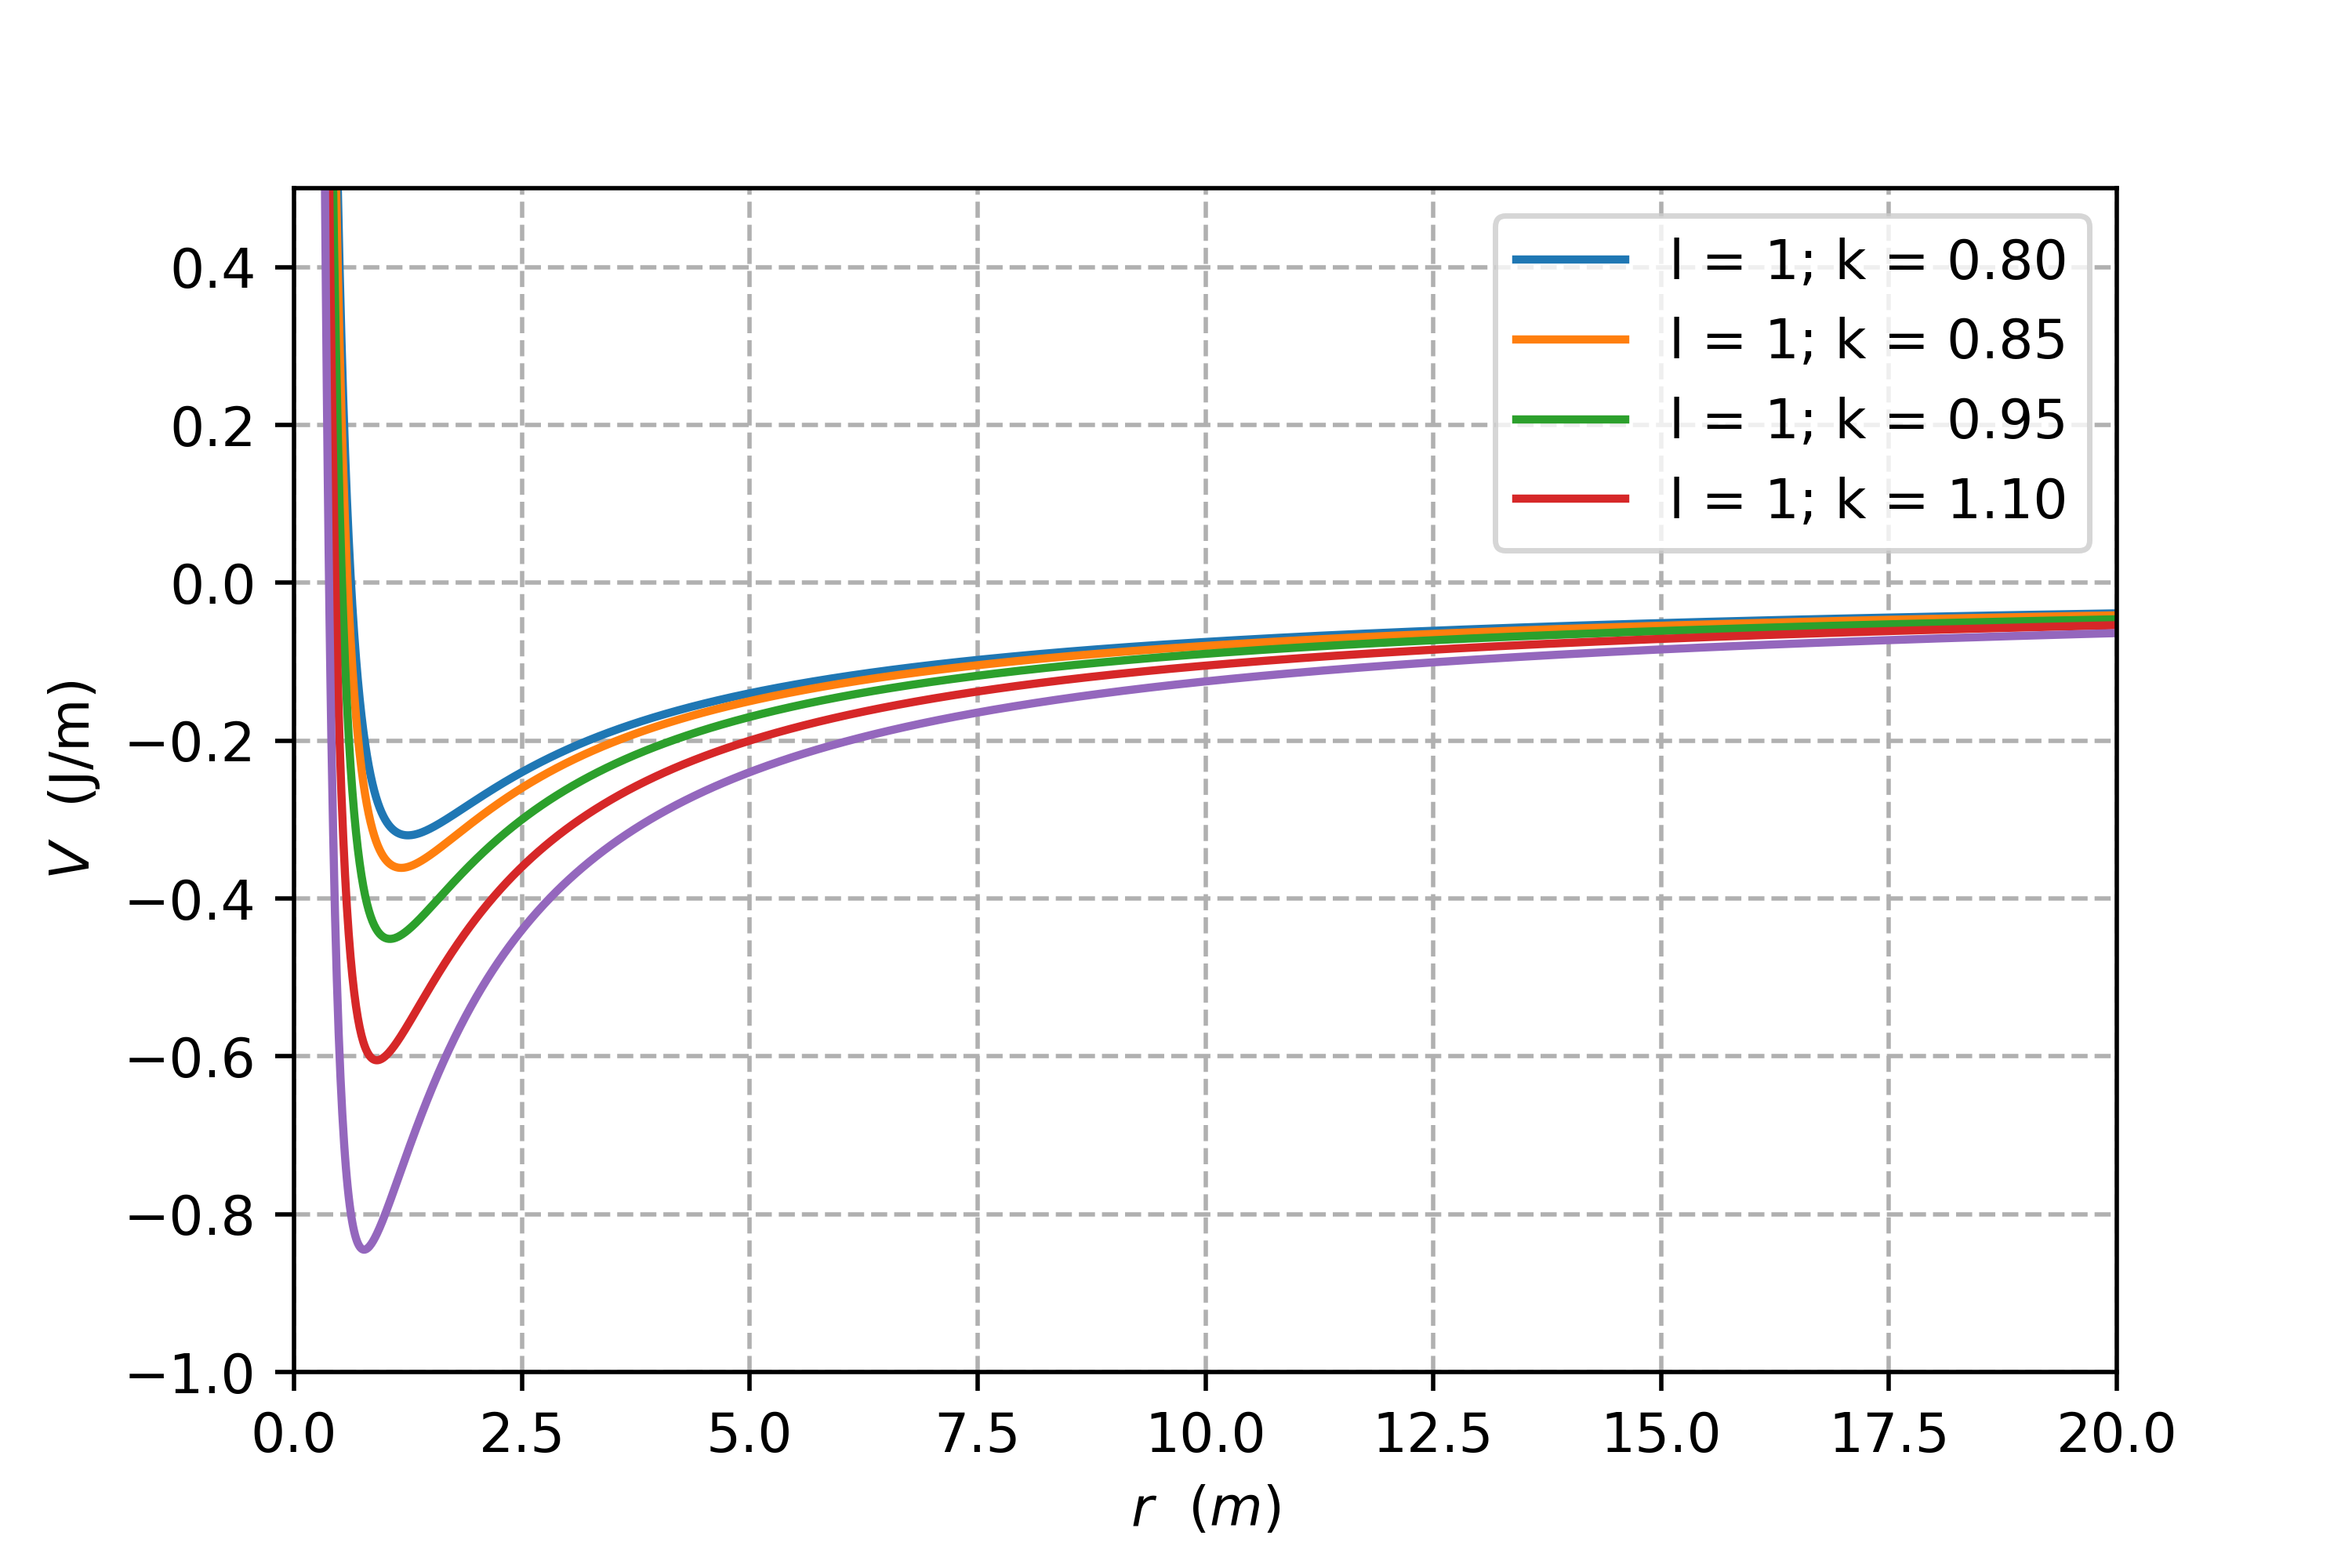
\includegraphics[scale=0.8]{gravedad_k.png}
\end{figure}

\begin{figure}[h!] \centering
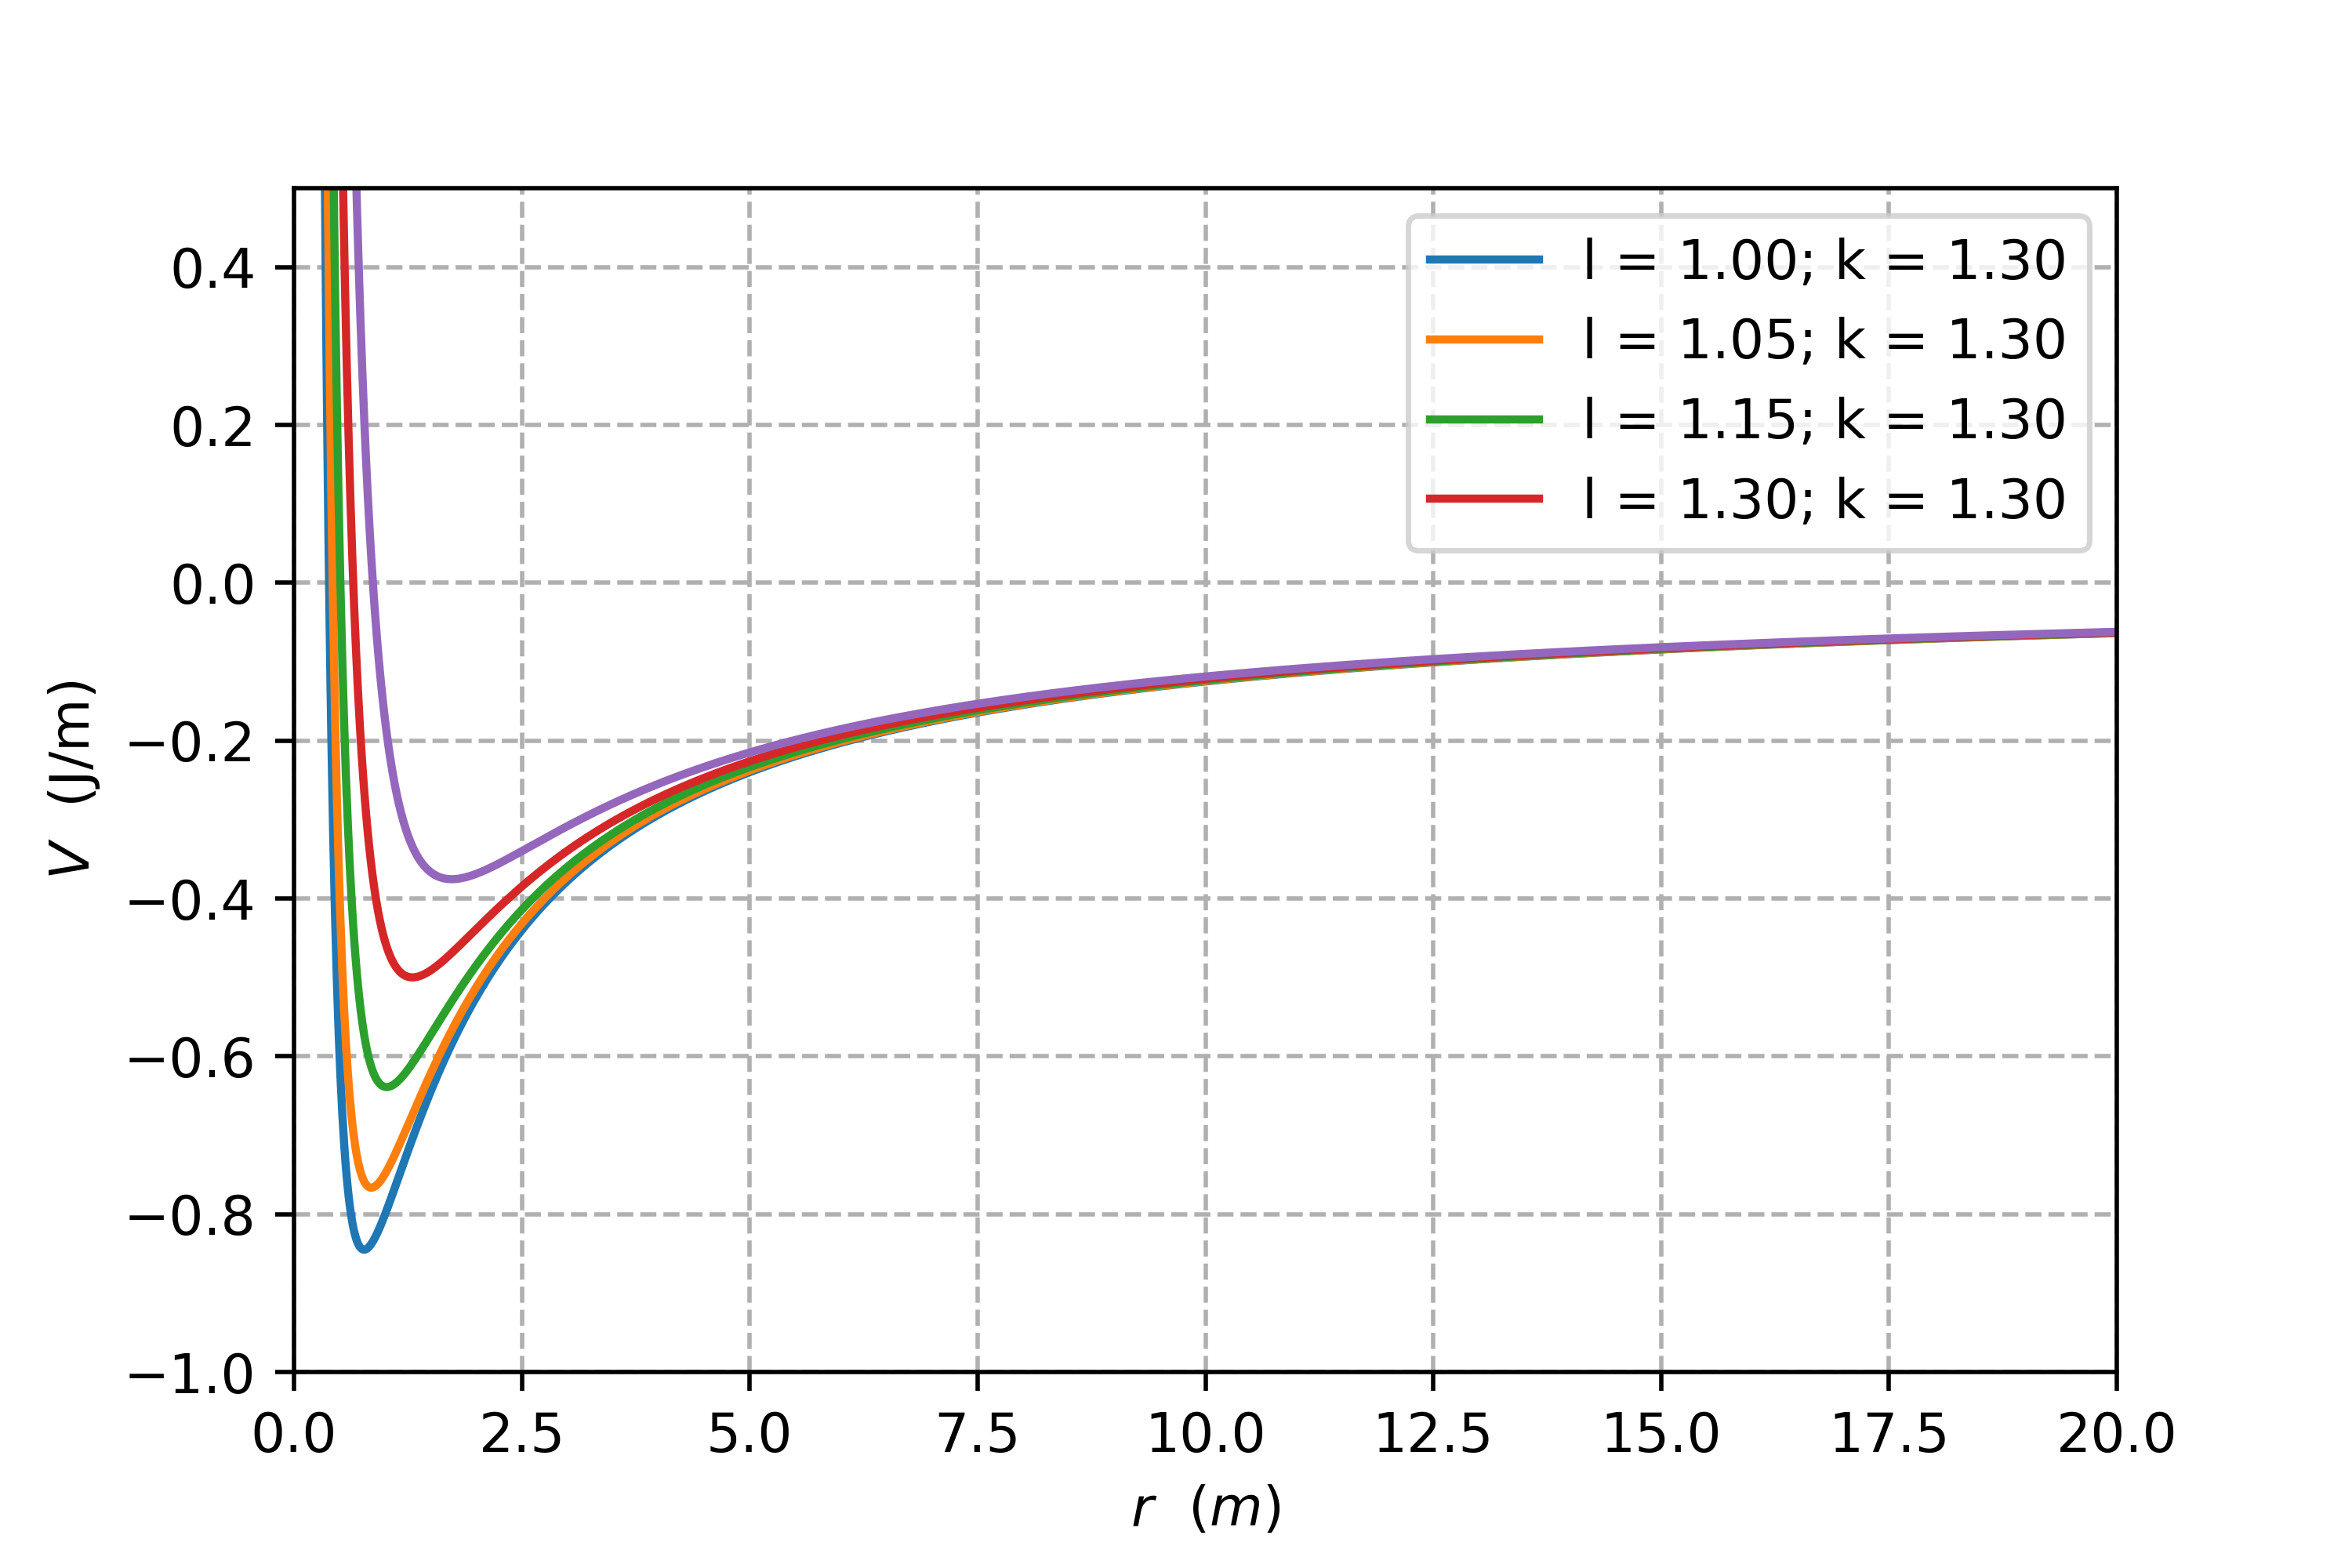
\includegraphics[scale=0.8]{gravedad_l.png}
\end{figure}


\subsection{Clasificación de las órbitas}

En función de la energía que lleve cierta masa podemos clasificar las órbitas cualitativamente, de manera muy sencilla. Si nos fijamos en la representación de un potencial efectivo, podemos ver que hay dos claras distinciones. Si $E \leq 0$ tenemos que la masa en cuestión va a poder ir hasta el infinito. Si $E=0$ tenemos que cuando llegue al infinito se quedará con velocidad $v=0$, y en el caso de que $E>0$ en el infinito conservará cierta velocidad. La otra posibilidad es que $E<0$. Si sucede esto pueden ocurrir dos cosas. Si $E=V_{\mathrm{min}}=E_0$ tenemos que la masa estara encerrada en una sola posible órbita, con un mismo radio constante. Si $V_{\mathrm{min}}<E<0$ podrá oscilar entre dos posibles radios, pero sin llegar a tender al infinito. Entendiendo esto podemos crear la siguiente clasificación:

\begin{itemize}
\item $E>0$. En este caso tendremos que la masa no estará acotada, de tal forma que si se acerca a el máximo de potencial, se ``dará la vuelta'', y se alejará infinitamente. Mas adelante estudiaremos que el movimiento se trata de una \textit{hipérbola}.

\item $E=0$. Tampoco estará acotada, de tal forma que le sucederá lo mismo que para $E>0$. Sin embargo en este caso cuando llegue al ``infinito'' no tendrá ningún tipo de velocidad. Su ecuación del movimiento será una \textit{parábola}.

\item $E_0<E<0$. El movimiento estará acotado entre dos posibles distancias $r_1$ y $r_2$, orbitando entorno al centro del potencial. Su ecuación del movimiento será una \textit{elipse}.

\item $E=E_0$. Estará restringido a un única distancia, por lo que $r=r_0=\alpha$ siempre. Está claro que su órbita será circular, ya que el único grado de libertad que posee es $\theta$. 
\end{itemize}

\subsection{Solución a la ecuación del movimiento}

La solución a la ecuación del movimiento se puede hacer por la manera integrar o mediante la ecuación de Binet. Como usando la ecuación de Binet la forma de deducirla es muchísimo mas sencilla y rápida, será la única que presentemos aquí. Tenemos que de la ecuación de Binet, si escribimos $F(r) = - k/r^2$ obtenemos que:

$$ \dfrac{\D}{\D \theta} \parentesis{\frac{1}{r}} + \dfrac{1}{r} = \dfrac{k \mu}{l^2} $$
Es fácil darse cuenta con el cambio de variables $p = 1/r$ que la solución es:

$$
p = \dfrac{1}{r} = A cos(\theta - \theta_0) + \dfrac{k \mu }{l^2}
$$
siendo $A$ y $\theta_0$ constantes de integración. Si definimos $\varepsilon$ como

\begin{equation}
\epsilon = \dfrac{A l^2}{\mu k} = A \alpha
\end{equation}
podemos escribir la ecuación del movimiento como:

\begin{equation}
r(\theta) = \dfrac{\alpha}{1 + \varepsilon \cos (\theta - \theta_0)}
\end{equation}
Ahora sabemos que en el radio mas pequeño posible de nuestra órbita tiene que verificarse que el denominador sera lo mas grande posible. Esto sucederá si $\theta-\theta_0$, por lo que si fijamos la constante $\theta_0 = 0$ tenemos que tener en cuenta que el radio mínimo se alcanzará cuando $\theta  =0 $ (ignorando los triviales múltiplos de $\pi$ y $2\pi$).

$$ r_{\mathrm{min}} = r(0) =  \dfrac{\alpha}{1+\epsilon}$$
En el punto donde $r_{\mathrm{min}}=r(0)$ tenemos que la energía total vendrá dada únicamente por el potencial:

$$ E = \dfrac{l^2}{2 \mu r^2(0)} - \dfrac{k}{r(0)} = \dfrac{k^2 (1+\epsilon)^2}{2 \mu \alpha^2} - \dfrac{k (1+\epsilon)}{\alpha} = \dfrac{k^2 \mu}{2 l^2} (\epsilon^2-1) $$
es decir, que $E$ y $\epsilon$ se relacionan tal que:

\begin{equation}
E = \dfrac{k^2 \mu}{2 l^2} (\epsilon^2-1) \quad \quad \quad \epsilon^2 = 1 + \dfrac{E 2 l^2}{\mu k^2}
\end{equation}

Si ahora estudiamos las ecuaciones del movimiento en cartesianas obtendremos que las ecuaciones del movimiento representan cónicas donde $\epsilon$ es la excentricidad de la órbita, siguiendo la clasificación anteriormente mencionada.

\subsection{Ecuaciones cartesianas}

Podemos escribir las ecuaciones del movimiento de manera cartesiana multiplicando por $1+\epsilon \cos \theta$ la ecuación del movimiento, y conociendo que $x=r \cos \theta$ y que $r=\sqrt{x^2+y^2}$, de tal forma que:

\begin{equation}
\sqrt{x^2+y^2} = \alpha - \epsilon x \label{Ec:2.2.4.01}
\end{equation}
La solución de cada ecuación no es sencilla, excepto para los casos donde $\epsilon = 0,1$. Saltándonos los pasos:

\begin{itemize}
\item \textbf{Órbitas circulares:} este tipo de órbitas se suceden si $\epsilon=0$, que es lo mismo que suponer que $E=E_0$. Como dijimos antes, en este caso las órbitas serán circulares de radio $\alpha$. 

\item \textbf{Órbitas elípticas:} este tipo de órbitas suceden si $0<\epsilon<1$, que es lo mismo que si $E_0 < E < 0$, como dijimos antes. Entonces la solución será:

\begin{equation}
\dfrac{(x^2 + \epsilon a)^2}{a^2} + \dfrac{y^2}{b^2} = 1
\end{equation}

donde $a$ es el semieje mayor y $b$ el semieje menor, que vienen dados por:

\begin{equation}
a = \dfrac{\alpha}{1-\epsilon^2} \quad \quad \quad b = \dfrac{\alpha}{\sqrt{1-\epsilon^2}}
\end{equation}

o también por:

\begin{equation}
a = - \dfrac{k}{2E} \quad \quad \quad b = \dfrac{l}{\sqrt{-2 \mu E}}
\end{equation}

La elipse estará centrada en ($ -\epsilon a, 0 $), y los focos serán (0,0) y ($-2a\epsilon,0$).

\item \textbf{Órbitas parabólicas:} suceden si $\epsilon = 1$ y llevan a que $E=0$. La ecuación del movimiento se de deduce de manera sencilla ya que si elevamos al cuadrado la ecuación \ref{Ec:2.2.2.01} tenemos que:

\begin{equation}
y^2 = \alpha^2 - 2 \epsilon \alpha x \Longrightarrow x = - \dfrac{y^2}{2 \alpha} + \dfrac{\alpha}{2}
\end{equation}

\item \textbf{Órbitas hiperbólicas:} este tipo de órbitas suceden si $\epsilon>1$, i.e. $E>0$, como ya hemos mencionado. La solución viene dada por: 

\begin{equation}
\dfrac{(x-\epsilon a)^2}{a^2} + \frac{y^2}{b^2} = 1
\end{equation}

donde los parámetros $a$ y $b$ vienen dados por:


\begin{equation}
a = \dfrac{\alpha}{\epsilon^2-1} \quad \quad \quad b = \dfrac{\alpha}{\sqrt{\epsilon^2-1}}
\end{equation}

o también por:

\begin{equation}
a = \dfrac{k}{2E} \quad \quad \quad b = \dfrac{l}{\sqrt{2 \mu E}}
\end{equation}

El resultado es una hipérbola centrada en el punto ($a \epsilon,0$) teniendo en cuenta uno de los focos en la origen de coordenadas. Las asíndotas serán $y=\pm \frac{b}{a}(x-a \epsilon)$. Cada una de las ramas corresponde un fenómeno físico diferente, una a un fenómeno en el que la fuerza atrae a la masa, y la otra a un fenómeno donde esta fuerza es de repulsión.

\end{itemize}

Por lo que hemos deducido claramente que $\epsilon$ es la excentricidad de la órbita. Es decir, la excentricidad depende de $E$, $l$, $k$ y $\mu$. 


\subsection{Leyes de Kepler}

Kepler fue un matemático y astrónomo alemán que se dedico toda su vida a estudiar el movimiento de los planetas. Siendo su obra mas notable la formulación de las leyes de Kepler, que hoy estudiamos deduciéndolas de la ley de gravitación de Newton, en realidad fue Newton quien basándose en estas dedujo su ley. Las leyes son:

\begin{itemize}
\item \textbf{Primera ley de Kepler:} los cuerpos celestes tienen movimientos elípticos alrededor del Sol, estando este en uno de los focos de la elipse. Llamamos \textit{perihelio} (\textit{perigeo} si hablamos de satélites terrestres) a la menor distancia que hay entre el sol y un planeta en su órbita, y \textit{afelio} (\textit{apogeo}) en el caso de la mayor distancia. Estas vienen dadas por:

\begin{equation}
r_{\mathrm{min}} = \dfrac{\alpha}{1+ \epsilon} = a (1 - \epsilon)  \quad \quad \quad
r_{\mathrm{max}} = \dfrac{\alpha}{1- \epsilon} = a (1 + \epsilon)
\end{equation}

\item \textbf{Segunda ley de Kepler:} la velocidad areolar es constante.

\begin{equation}
\dfrac{\D A}{\D t} = \dfrac{l}{2 \mu}
\end{equation}

\item \textbf{Tercera ley de Kepler:} el cuadrado del periodo de las órbitas de los planetas guarda proporción con el cubo de la distancia que hay con el sol. Usando la segunda ley de Kepler podemos deducir que el periodo en el que tarda en dar una vuelta al sol un planeta barre toda el área (siendo el área de una elipse $\pi a b$). Entonces si:

\begin{equation}
T = \dfrac{2 \mu}{l} \pi a b \Longrightarrow T^2 = \dfrac{4 \pi^2}{G (m_1 + m_2)} a^3
\end{equation}

\end{itemize}

\section{Colisiones. Secciones eficaces}

Los experimentos de colisiones son extremadamente importantes para la física, sobretodo para la física cuántica. Los experimentos de \textit{scattering} (colisiones o dispersión) permiten obtener información de una colisión entre dos partículas u objetos a partir de dos el ángulo con el que sale el objeto tras la colisión (o los objetos) y el parámetro de impacto, que es una especie de medida de la puntería, aunque realmente no es así. Definiendolos de manera rigurosa:

\begin{itemize}
\item  \textbf{Ángulo de dispersión:} es el ángulo que forma la dirección que entra y la dirección que sale del objeto estudiado. Se denota por $\theta$.
\item \textbf{Parámetro de impacto:} es la distancia perpendicular entre los objetos que colisionan.
\end{itemize}

En general los problemas de scattering tratan de calcular la relación entre $\theta$ y $b$, calculando $b(\theta)$ o $\theta(b)$. 

\subsection{Sección eficaz de colisión}

Definimos sección eficaz como el área efectiva a partir la cual los objetos interactuen.
Sea $A$ el área total del conjunto de partículas que están quietas (las que reciben el objeto que colisiona), y $n_b$ el número de estas partículas por unidad de superficie. Si $\sigma$ es el área eficaz, es decir, el área que tiene el objeto lanzado para interactuar con las partículas, tenemos que el número de proyectiles que chocarán contra alguna partícula $N_{sc}$ será

\begin{equation}
N_{sc} = N_{inc} \dfrac{n_b \sigma A}{A}
\end{equation}
donde $N_{inc}$ es el número de proyectiles incidentes. A esta relación se llama la \textbf{relación fundamental de la teoría de colisiones}  Conociendo $N_{sc}, N_{inc}, n_b$ podremos conocer entonces la sección eficaz $\sigma$. \\

La sección eficaz de una colisión depende principalmente de dos factores: la superficie del objeto y del tipo de interacción. Obviamente cuanto mayor sea la superficie del objeto habrá mas probabilidad de que haya una colisión entre ellos. Además de este factor el tipo de interacción también afectara a la trayectoria. Por ejemplo, si lanzamos un electrón a un protón este último repelerá al electrón, por lo que realmente la sección eficaz, la superficie de colisión es mucho menor. En general este tipo de interacciones necesitan una mayor puntería. Sin embargo si lanzamos una masa hacia la tierra, está se vera atraía (por la fuerza gravitatoria), por lo que podremos tener menos puntería, y acertaríamos igual (acertar equivale a la existencia de una interacción).\\
 
Es un gran ejemplo el que presenta Jose Manuel Sanchez de Santos en sus apuntes: ``\textit{Imaginemos una diana trucada que atrae a los dardos. Está claro que con un parámetro de impacto mayor será suficiente para acertar en la diana. Esta parece mas grande de lo que es en realidad: la sección eficaz es mas grande que la superficie de la diana (sección eficaz mayor). Si la diana repeliese los dardos la situación sería la contraria: aun con buena puntería será difícil acertar con el dardo en la diana, que aparenta ser mas pequeña (sección eficaz menor)}''. \\

En general en los experimentos reales distinguimos dos tipos de colisiones:

\begin{itemize}
\item Colisión elástica: en estas colisiones normalmente se mantiene el proyectil íntegramente.
\item Colisión inelástica: en estas colisiones las partículas se funsionan, intercambian masa...
\end{itemize}

\subsection{Sección eficaz diferencial}


Como ya hemos visto, la sección eficaz de antes tiene en cuenta únicamente la interacción, y no como interactúan, es decir, en que dirección son dispersadas, con que parámetro de impacto colisionan...  Entonces para esto tendremos que definir la \textbf{sección eficaz diferencial}, que es basicamente el número de partículas que se dispersan en un cono estrecho, lo que se suele entender como un elemento de ángulo sólido. \\

\begin{figure}[h!] \centering
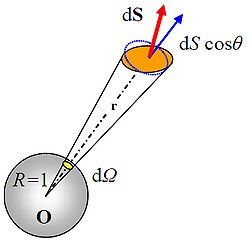
\includegraphics[scale=1]{angulosolido.jpg}
\end{figure}


Si llamamos a $\Omega$ el ángulo sólido, entendiendo elemento de ángulo sólido como \begin{equation}
\D \Omega = \sin \theta \D \theta \D \phi \label{Ec:2.1.2.01}
\end{equation}
podemos relacionar mediante la relación fundamental el número de partículas dispersadas en un elemento de ángulo sólido:

$$ \D N_{sc} = N_{inc} n_b \D \sigma $$

entonces está claro que la sección eficaz diferencial está relacionada con el elemento de ángulo sólido de tal manera que:

\begin{equation}
\D \sigma (\phi, \theta) = \frac{\D \sigma}{\D \Omega} (\phi, \theta) \D \Omega
\end{equation}

Donde el factor siguiente es la llamada \textbf{sección eficaz diferencial}:

\begin{equation}
\frac{\D \sigma}{\D \Omega} (\phi, \theta)
\end{equation}

Ahora vamos a relacionar la sección eficaz relacionar con el ángulo de scattering y el parámetro de impacto. Entonces si el ángulo sólido está centrado en el ángulo de dispersión $\theta$, y $b$ es el parámetro de impacto para el cual sale el proyectil con esa dispersión. Tenemos que para dicho ángulo de dispersión tendremos unas áreas que se relacionan como:

\begin{equation}
\D \sigma = 2 \pi b \D b
\end{equation}

tal y como se puede ver en la figura:

Además $\theta$ y $\Omega$ están relacionados ya que según la ecuación \ref{Ec:2.1.2.01} tenemos que:

\begin{equation}
\D \Omega = 2 \pi \sin(\theta) \D \theta
\end{equation}

Entonces podemos relacionar la sección eficaz diferencial con la derivada de $b$ y $\theta$, de tal manera que:

\begin{equation}
\frac{\D \sigma}{\D \Omega} = \dfrac{b}{\sin \theta} \left| \frac{\D b}{\D \theta} \right|
\end{equation}

El valor absoluto es importante ya que a veces la derivada entre $b$ y $\theta$ es negativa y obviamente la derivada de la izquierda no lo es. 



% AÑADIR FOCOS, DISTANCIAS, ETC PARA LAS CONICAS. EXPRESIONES COMO LAS DE LA DIFERENCIA DE VELOCIDAD PARA UNA ELIPSE (COMO EJEMPLOS). EJEMPLOS DE EJERCICIOS PARA LAS PARABOLAS/HIPERBOLAS/ELIPSES. EXPRESIONES QUE NOS AYUDEN A CALCULAR UN RADIO DE LA ELIPSE CONOCIENDO EL OTRO. 

\chapter{Mecánica del cuerpo rígido}

Un cuerpo rígido es un sistema de puntos materiales sometidos a ligaduras holónomas consistentes en que las distancia entre dos puntos del sistema se mantienen constantes durante el movimiento. Así que en este capítulo estudiaremos su movimiento, su naturaleza. Además estudiaremos un poco que son los tensores, lo cual será muy útil para estudios físicos fuera de la mecánica clásica.

\section{Grados de libertad}

Antes de empezar a estudiar el movimiento de un cuerpo rígido debemos saber cuántos grados de libertad posee nuestro problema. Como sabemos una partícula posee 3 grados de libertad, entonces un sistema de N partículas tendrá 3N grados de libertad. Sin embargo para definir con exactitud la posición de una partícula solo es necesario conocer la distancia a 3 partículas con vectores posición linealmente independientes, es decir, que no estén alineados. Entonces tendremos 9 grados de libertad, que se reducen a 6 grados ya que existen 3 ligaduras holónomas entre ellas, tenemos que en realidad hay 6 grados de libertad en nuestro sistema. \\

Goldstein nos explica que que solo haya 6 grados de libertad puede tener la siguiente implicación: primero establecemos la posición de uno de los puntos del problema, que poseerá 3 grados de libertad. Luego podemos especificar el segundo punto por dos coordenadas, ya que al tener que estar a la misma distancia del punto 1 se moverá sobre una superficie esférica alrededor de este. El punto 3 se puede especificar con una sola coordenada, ya que solo puede girar alrededor de un punto que une los otros dos puntos.  Por eso son suficientes 6 grados de libertad. \\

Entonces un cuerpo rígido necesita 6 coordenadas generalizadas independientes para especificar su posición, con independencia del tamaño, número de partículas y forma. Ahora bien, ¿Cómo se asignan dichas coordenadas? Bueno, pues en realidad es bien sencillo. Si suponemos que existe un eje de coordenadas cartesiano fijo en un punto del cuerpo está claro que la posición de este estará especificado con 3 coordenadas que nos indiquen la posición del origen de coordenadas respecto el sistema de coordenadas externo. Las otras 3 coordenadas especificarán la orientación de los ejes respecto al otro sistema.  Así podemos especificar cada eje de coordenadas con una rotación, de tal forma que:

\begin{equation}
\begin{array}{lll}
\widehat{i} ' & = & \widehat{i} \cos  \alpha_1 + \widehat{j} \cos  \alpha_2 + \widehat{k} \cos \alpha_3 \\ \\
\widehat{j} ' & = & \widehat{i} \cos  \beta_1 + \widehat{j} \cos  \beta_2 + \widehat{k} \cos \beta_3 \\ \\
\widehat{k} ' & = & \widehat{i} \cos  \delta_1 + \widehat{j} \cos  \delta_2 + \widehat{k} \cos \delta_3
\end{array}
\end{equation} 

$$ \Longrightarrow $$

\begin{equation}
\begin{pmatrix}
\widehat{i}' \\
\widehat{j}' \\
\widehat{k}' \\
\end{pmatrix}
=
\begin{pmatrix}\cos(\alpha_{1}) &
\cos(\alpha_{2}) &
\cos(\alpha_{3}) \\ 
\cos(\beta_{1}) &
\cos(\beta_{2}) &
\cos(\beta_{3}) \\ 
\cos(\delta_{1}) &
\cos(\delta_{2}) &
\cos(\delta_{3}) \\ 
\end{pmatrix}
\begin{pmatrix}
\widehat{i} \\
\widehat{j} \\
\widehat{k} \\
\end{pmatrix}
\end{equation}

$$ \Longrightarrow $$



\begin{equation}
\begin{pmatrix}
\widehat{i}' \\
\widehat{j}' \\
\widehat{k}' \\
\end{pmatrix}
=
\begin{pmatrix}
a_{1 1 } &
a_{1 2 } &
a_{1 3 } \\ 
a_{2 1 } &
a_{2 2 } &
a_{2 3 } \\ 
a_{3 1 } &
a_{3 2 } &
a_{3 3 } 
\end{pmatrix}
\begin{pmatrix}
\widehat{i} \\
\widehat{j} \\
\widehat{k} \\
\end{pmatrix} \label{Ec:3.3-matrizcambiobase1}
\end{equation}

Estos nueve cosenos directores nos permiten definir la trasformación entre los dos sistemas de coordenadas. En este sentido los ángulos nos describen la orientación instantánea del cuerpo respecto a un sistema de coordenadas fijo en el espacio, pero con origen común con el sistema del cuerpo. Sin embargo está claro que no pueden ser independientes: solo hay 3 grados de libertad angulares. Las ligaduras que reducen los ángulos provienen del hecho de que son coordenadas ortogonales entre sí, y tienen módulo unidad, de tal manera que las ecuaciones son:

\begin{equation}
\begin{array}{l}
i' \cdot j' = j' \cdot k' = k' \cdot i'  = 0 \\ \\
i' \cdot i' = j' \cdot j' = k' \cdot k' = 1 
\end{array}
\end{equation}

Esto nos reduce el problema a la existencia de 9 ángulos y cosenos directores a 3 coordenadas angulares independientes, como habíamos deducido antes. A esta trasformación la conocemos como \textbf{cambio de base ortonormal}. De hecho todo el problema de la mecánica de un sólido rígido (y la mitad del problema de la mecánica clásica, ya que la otra mitad son las traslaciones), que se basa en las rotaciones. Son tan sumamente importantes que vamos a estudiar toda una sección que nos permita entender las rotaciones de cualquier tipo como la suma de las rotaciones de ejes. 





\section{Rotaciones}

\subsection{Convenio de Einstein}
En el cálculo tensorial y matricial aparecen constantemente sumatorios de algún índice. Einstein, cuando trataba de escribir su teoría de la relatividad se cansó de escribir sumatorios e índices, por lo que introdujo lo que hoy conocemos como \textit{convenio de Einstein} para la suma de índices. Entonces se entenderá que siempre qeu haya dos índices repetidos habrá una suma de dicho índice de todos los valores posibles. Ejemplos:

$$
\begin{array}{lll}
x_i' = \sum_{i=1}^3 a_{ij} x_j
 & \longrightarrow  & x_i' = a_{ij} x_j  \\ \\
 
 \vec{x} \cdot \vec{y} = \sum_{i=1}^3 x_i y_i & \longrightarrow & \vec{x} \cdot \vec{y} = x_i y_i
\end{array} 
$$
Los índices repetidos se llaman \textit{indices mudos} y los no repetidos \textit{indices libres}.

\subsection{Cambio de base ortonormal}
 Sea $A$ la matriz cambio de base, que será exactamente análoga a la de la ecuación \ref{Ec:3.3-matrizcambiobase1}:

\begin{equation}
A = \begin{pmatrix}
a_{1 1 } &
a_{1 2 } &
a_{1 3 } \\ 
a_{2 1 } &
a_{2 2 } &
a_{2 3 } \\ 
a_{3 1 } &
a_{3 2 } &
a_{3 3 } 
\end{pmatrix}
\end{equation} 
 Por lo que podemos escribir que la notación en los ejes primados y la notación en los ejes originales viene dada por la relación:
 
\begin{equation}
\vec{r'} =  A  \cdot \vec{r}
\end{equation}

Esto tiene un significado bastante profundo: al operar la matriz $A$ sobre las componentes de un vector en el sistema original no estamos cambiando el vector, este permanece \textit{inalterado}. Sólo estamos buscando sus componentes en dos sistemas de coordenadas. En un plano esto supondría hacer girar al vector $\vec{r}$ un ángulo $\phi$, dando un nuevo vector $\vec{r}'$. Podemos interpretarla como una operación sobre el sistema de coordenadas o como una operación que actúa sobre el vector. La interpretación como operador que actúa sobre las coordenadas será mas pertinente cuando se utilice como transformación ortogonal para especificar la orientación del cuerpo rígido. Sin embargo si posee una dualidad. A veces puede considerarse que sólo afectan al sistema de coordenadas, expresando alguna cantidad o función dada en un nuevo sistema de coordenadas. En otras ocasiones se puede considerar que operan sobre la propia cantidad o función, trasformándolas en nuevas cantidades enel mismo sistema de coordenadas. En el primer caso hablamos del papel \textit{pasivo}, en el segundo del papel \textit{activo} (la trasformación altera un vector o otra magnitud) del operador.\\

\begin{equation}
A^{T} = A^{-1} \Longrightarrow A^T A = \mathds{1} \label{Ec:3.10}
\end{equation}


\begin{equation}
\vec{r} = A^T \cdot \vec{r'}
\end{equation} 
De la ecuación \ref{Ec:3.10} se pueden deducir las siguientes condiciones:

\begin{equation}
\sum_{i=1}^3 \sum_{j=1}^3 a_{ki} a_{lj} = \delta_{kl}
\end{equation}
que son 6 relaciones independientes de ortogonalidad, que verifican lo que vimos en el apartado anterior. Para una trasformación ortogonal tenemos que:

$$ A \cdot A^T = \mathds{1} \Longrightarrow (\Det (A))^2 = 1 \Longrightarrow \Det (A) = \pm 1 $$

Entonces llamamos \textbf{trasformaciones propias} a aquellas que su determinante es 1 y \textbf{transformaciones impropias} si son negativas. A cada signo de la transformación podemos asignarle un significado físico diferente. 1. Sin embargo, el
razonamiento siguiente demuestra que una matriz ortogonal cuyo determinante valga — 1
no puede representar un desplazamiento físico de un cuerpo rígido. Consideremos la siguiente matriz:

$$ S = \begin{pmatrix}
-1 &
0 & 
0 \\
0 & 
-1 &
0 \\
0 & 
0 & 
-1 
\end{pmatrix} $$

Dicha trasformación cambia el signo de cada una de las componentes de los ejes de coordenadas. Tal operación trasforma el un sistema de coordenadas \textit{dextrógiro} en un \textit{levórgiro}, y se denomina \textit{inversión} de los ejes de coordenadas. Véase figura \ref{Fig:3.1}. \\



\begin{figure}[h!] \centering
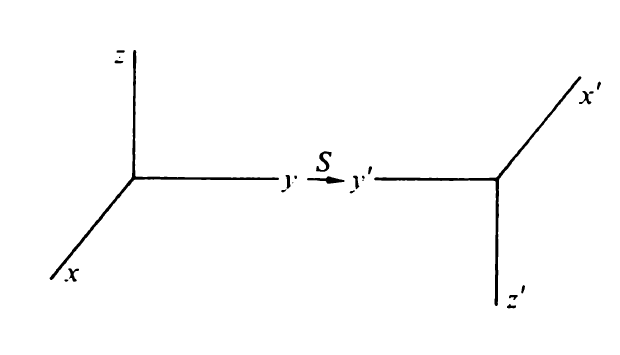
\includegraphics[scale=1]{inversionejes.png}
\caption{inversion de los ejes de coordenadas}
\label{Fig:3.1}
\end{figure}

Por la misma naturaleza de esta operación, queda claro que la inversión de un sistema dextrogiro en otro levogiro no puede lograrse mediante ningún cambio rígido de orientación de los ejes de coordenadas. Por tanto, una inversión no corresponderá nunca a un desplazamiento físico de un cuerpo rígido. Lo que es cierto para S lo será igualmente para toda matriz cuyo determinante valga - 1, ya que dicha matriz se puede escribir en forma de producto de S por una matriz cuyo determinante valga un número positivo, y por tanto incluye la operación de inversión. En consecuencia, no podrá describir un cambio de orientación rígido. Por tanto, las transformaciones que representen el movimiento de un cuerpo rígido deberán limitarse a matrices cuyo determinante valga +1. Otro método para llegar a esta conclusión parte del hecho de que la matriz de cambio debe evolucionar de manera continua a partir de la matriz unidad la cual, desde luego, tiene +1 por determinante. Sería incompatible con la continuidad del movimiento que el determinante de la matriz cambiase repentinamente, en algún instante, de su valor inicial +1 a -1. \\


\subsection{Ángulos de Euler}

Para describir el movimiento de cuerpos rígidos en la formulación de Lagrange de la
Mecánica será, pues, necesario buscar tres parámetros independientes que especifiquen la orientación de un cuerpo rígido de tal manera que la matriz ortogonal de cambio correspondiente tenga su determinante igual a +1. A lo largo de la historia se han descrito algunos conjuntos de parámetros, aunque el mas corriente y útil lo constituyen los \textbf{ángulos de Euler}. Vamos a definir estos ángulos y como se puede expresar en función de ellos los elementos de la matriz ortogonal de cambio. \\

Podemos efectuar la trasformación de un sistema de coordenadas a otro por medio de tres rotaciones sucesivas efectuadas en un orden concreto. Se definen como ángulos de Euler como los tres ángulos de rotación sucesivos. Aunque la eleccion de los ángulos de rotación es libre, el convenio que vamos a ver es el mas usado.

\begin{figure}[h!] \centering
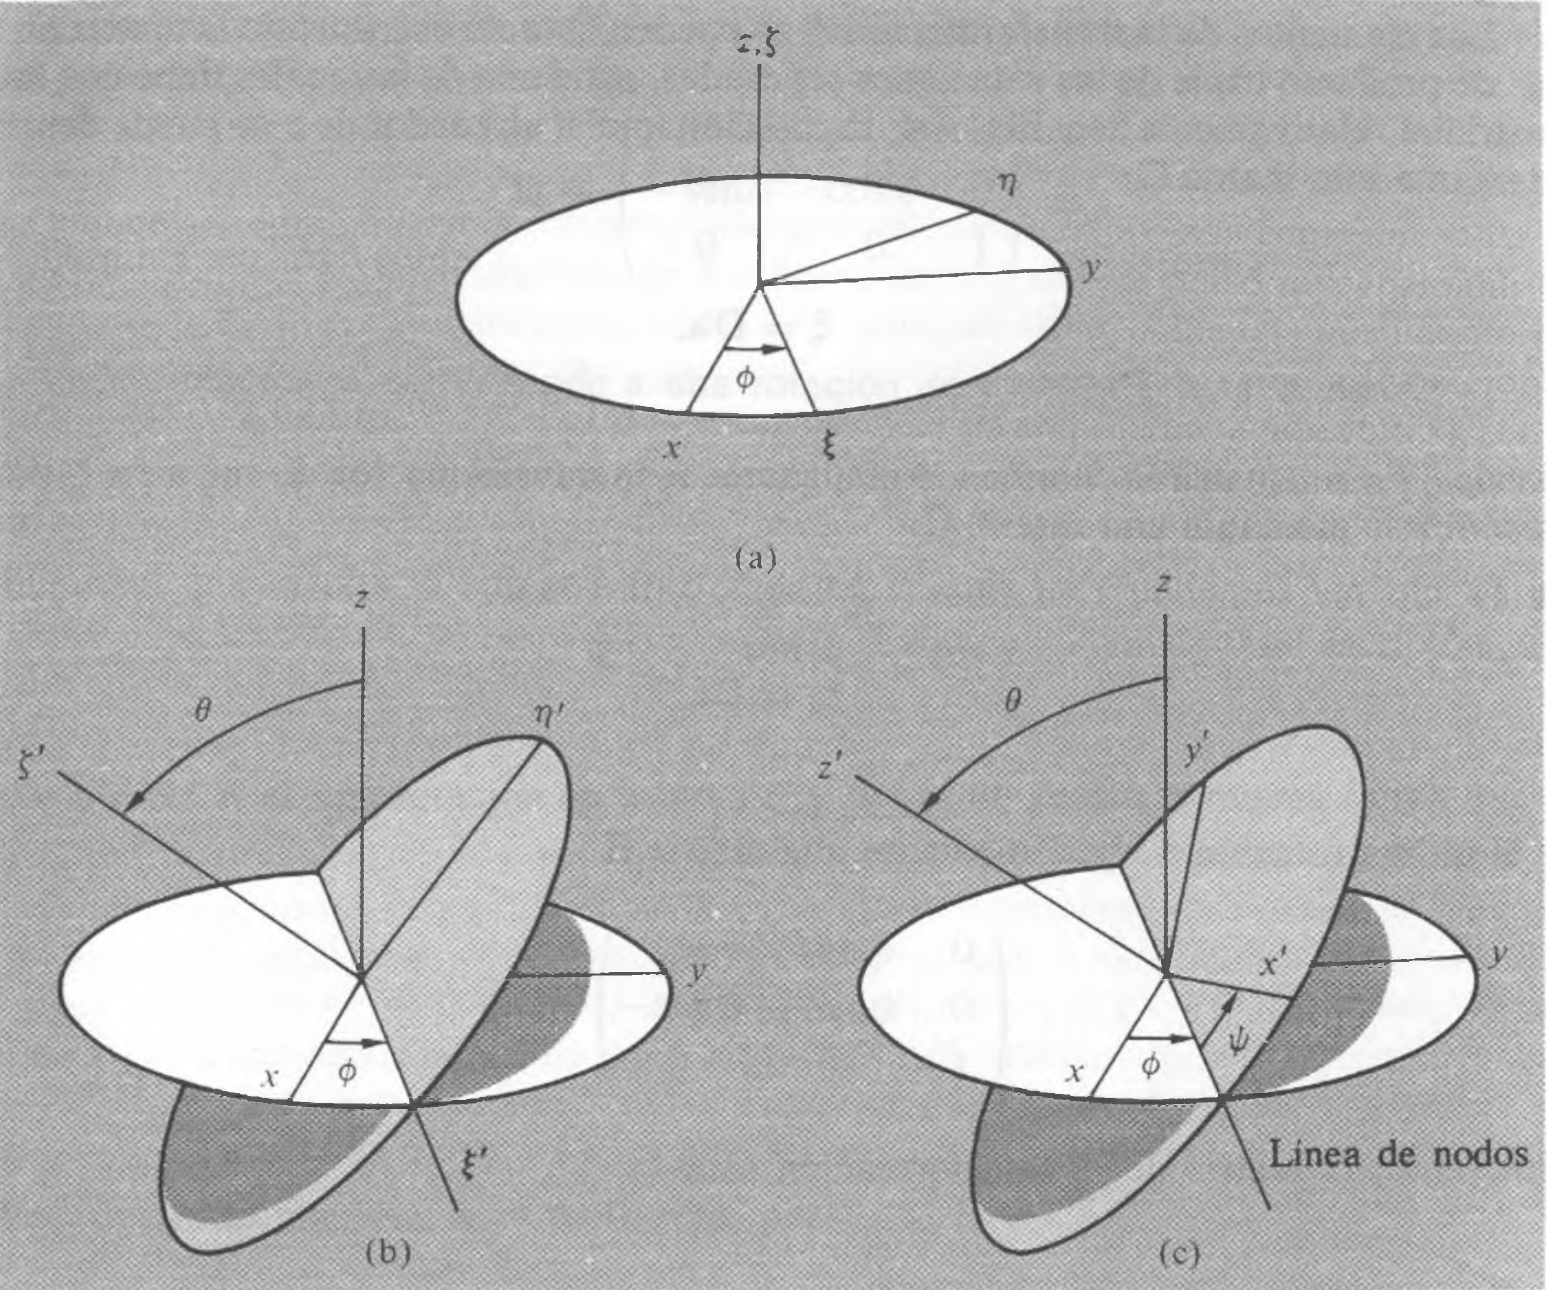
\includegraphics[scale=0.6]{anguloseuler.png}
\caption{Rotaciones que definen a los ángulos de Euler}
\end{figure}

El orden que vamos a emplear se inicia haciendo girar haciendo el sistema de ejes $xyz$ un ángulo $\phi$ alrededor del eje $z$ en sentido antihorario, tal y como aparece en la figura a), rotulando a los ejes del nuevo sistema de coordenadas como $ \xi \eta \varsigma$. En la segunda etapa se hace girar los ejes intermedios, un ángulo $\theta$ en sentido antihorario para dar lugar a otro sistema intermedio: $\xi' \eta' \varsigma'$. Véase la figura b). Por último, los ejes $\xi' \eta' \varsigma'$ se hacen girar en sentido antihorario un ángulo $\psi$ de tal manera que se crean los ejes $x'y'z'$. Así pues los ángulos $\theta, \phi, \psi$ son los que especifican totalmente la orientación de $x'y'z'$ respecto al $xyz$, y pueden ser por tanto las tres coordenadas generalizadas necesarias. \\

Los elementos de la trasformación ortogonal $A$ se pueden obtener escribiendo la matriz en forma de producto triple de las rotaciones separadas, cada una de las cuales tiene una forma matricial relativamente sencilla. Así la rotación inicial alrededor de $z$ se puede describir mediante una matriz D:

$$ \xi = D x $$

Donde $\eta$ y $x$ son matrices columna. Análogamente, la segunda trasformación puede describirse mediante una matriz C:

$$ \xi ' = C \xi $$
y la última rotación a $x'y'z'$ se puede hacer mediante una matriz $B$:

$$ x' = B \xi' $$
entonces tenemos que la trasformación total:

$$ x' = A x $$
siendo $A$ el producto de las matrices sucesivas:

\begin{equation}
A = B \cdot C \cdot D
\end{equation}
Ahora tenemos que ver exactamente como funciona cada una de las rotaciones. La trasformación D es rotación alrededor del eje $z$. La segunda trasformación es una trasformación respecto al eje $\xi$ y la última trasformación es una rotación en torno a $\varsigma'$ por lo que tendrá la misma forma que $D$:

\begin{equation}
D = \begin{pmatrix}
1 &
0 &
0 \\ 
0 &
\cos(\theta) &
\sen(\theta) \\ 
0 &
-\sen(\theta) &
\cos(\theta) \\ 
\end{pmatrix}
\end{equation}

\begin{equation}
C = \begin{pmatrix}
\cos(\phi) &
\sen(\phi) &
0 \\ 
-\sen(\phi) &
\cos(\phi) &
0 \\ 
0 &
0 &
0 \\ 
\end{pmatrix}
\end{equation}

\begin{equation}
B = \begin{pmatrix}
\cos(\psi) &
\sen(\psi) &
0 \\ 
-\sen(\psi) &
\cos(\psi) &
0 \\ 
0 &
0 &
0 
\end{pmatrix}
\end{equation}


Si hacemos la multiplicación:

\begin{equation}
A = \begin{pmatrix}
\cos \psi \cos \phi -  \cos \theta \sin \phi \sin \psi & \cos \psi \sin \phi -  \cos \theta \cos \phi \sin \psi & \sin \psi \sin \theta \\
\cos \psi \cos \phi -  \cos \theta \sin \phi \sin \psi & \cos \psi \cos \phi -  \cos \theta \sin \phi \sin \psi & \cos \psi \sin \theta \\
\sin \theta \sin \phi & - \sin \theta \cos \phi & \cos \theta 
\end{pmatrix}
\end{equation}

siendo la trasformación inversa:

\begin{equation}
x = A^{-1} x' = A^T x'
\end{equation}

El orden de rotaciones utilizado para definir la orientación final del sistema de coordenadas es, hasta cierto punto, aribitrario. La rotación inicial podría tomarse en torno a cualquiera de los tres ejes cartesianos. En las tres rotaciones lo único que no puede haber es dos rotaciones seguidas entorno al mismo eje. \\

Las velocidades asociadas a cada uno de los ejes también sufren por la matriz de cambio. Como podemos observar:

\begin{equation}
\vec{w}_{\phi} = \begin{pmatrix}
0\\
0\\
\dot{\phi}
\end{pmatrix}_{xyz}; \tquad \vec{w}_\theta = \begin{pmatrix}
\dot{\theta} \\
0\\
0
\end{pmatrix}_{\xi,\eta,\varsigma}; \tquad \vec{w}_\psi = \begin{pmatrix}
0\\
0\\
\dot{\psi}
\end{pmatrix}_{\xi', \eta', \varsigma'}
\end{equation}

Si sumamos las tres componentes de obtenemos que:

\begin{equation}
\vec{w} = BC \vec{w}_\phi + B \vec{w}_\theta + \vec{w}_\psi = \begin{pmatrix}
\dot{\phi} \sin \theta \sin \psi + \dot{\theta} \cos \psi \\
\dot{\phi} \sin \theta \cos \psi - \dot{\theta} \sin \psi \\
\dot{\phi} \cos \theta + \dot{\psi}
\end{pmatrix} = \begin{pmatrix}
w_{x'} \\
w_{y'} \\
w_{z'}
\end{pmatrix} \label{Ec:3.1-017}
\end{equation}

\subsection{Teorema de Euler y Chasles}

Lo visto en este apartado proporciona una técnica matemática completa para describir los movimientos de un cuerpo rígido. En todo instante la orientación del  cuerpo se puede concretar mediante una transformación ortogonal, cuyos elementos se pueden expresar en función de un sistema adecuado de parámetros. Al transcurrir el tiempo, la orientación variará y por tanto la matriz de cambio va a cambiar. Como el movimiento físico es continuo $A(t)$ debe ser una función continua  del tiempo, y en el instante inicial los ejes del cuerpo son coincidentes con los ejes espaciales tenemos que $A$ será la matriz identidad. Entonces la trasformación evoluciona \textit{cotinuamente a partir de la transformación identidad}. Con este método ya estamos en condiciones de obtener las características mas importantes del movimiento del cuerpo rígido, siendo de importancia fundamental el siguiente teorema:

\begin{theorem}[Teorema de Euler]
el corrimiento general de un cuerpo rígido con un punto fijo es una rotación alrededor de un cierto eje. 
\end{theorem}

El teorema dice entonces que el sistema de ejes del cuerpo se puede obtener en todo instante $t$ como una rotación del sistema de ejes inicial. Dicho de otro modo la \textit{operación} implícita en la matriz $A$ que describe el movimiento físico del cuerpo rígido es una \textit{rotación}. Un corolario directo del teorema de Euler es:

\begin{theorem}[Teorema de Chasles]
el corrimiento más general de un cuerpo rígido es una traslación mas una rotación
\end{theorem}


\subsection{Rotaciones infenitesimales}

Ahora que hemos establecido que se puede obtener cualquier orientación dada mediante una sola rotación en torno a un eje determinado, nos sentimos tentados de intentar asociar un vector (vector director del eje) de tal manera que quede fijo en la rotación. Sin embargo una rotación completa no puede hacerse considerando un eje fijo: como podemos ver hay rotaciones en la que cambian los tres ejes. Sin embargo esto si se cumple para \textbf{rotaciones infinitesimales}. Una rotación infinitesimal es una trasformación ortogonal de ejes de coordenadas en la cual las componentes de un vector son casi iguales en los dos sistemas de ejes (cambio infinitesimal). En notación matricial se puede escribir como:

$$ x' = (\mathds{1} + \Lambda ) x = A x $$
donde claramente se puede escribir en notación no matricial:

$$ x'_1 = x_1 + \lambda_{11} x_1 + \lambda_{12} x_2 + \lambda_{13} x_3 $$ 
La matriz inversa para la trasformación infinitesimal se obtiene fácilmente como:

$$A^{-1} = \mathds{1} - \Lambda$$
y si consideramos que:

$$ A \cdot A^{-1} = (\mathds{1} - \Lambda)(\mathds{1} + \Lambda)=\mathds{1} - \Lambda^2 = \mathds{1}  $$
para que esto se cumpla la matriz infinitesimal tiene que ser antisimétrica. Esto es porque $|A|=1$ (condicion de ortonormalidad), y esto solo ocurre si $\Lambda$ es antisimétrica. Los elementos diagonales de la matriz antisimétrica tienen que ser 0 (ya que si no $| \Lambda | = 1$. Podemos escribir $\Lambda$ de la siguiente forma sin perder generalidad:

\begin{equation}
\Lambda = \begin{pmatrix}
0 &
-\D \Omega_3 &
\D \Omega_2 \\ 
\D \Omega_3 &
0 &
-\D \Omega_1 \\ 
-\D \Omega_2 &
\D \Omega_1 &
0 \\ 
\end{pmatrix}
\end{equation}

Estas tres cantidades está claro que deben identificarse con los tres parámetros independientes que especifican la relación. Como $$\D x = x' - x = \Lambda x$$ de manera desarrollada podemos escribir:

\begin{equation}
\begin{array}{ll}
\D x_1 = & x_3 \D \Omega_2 - x_2 \D \Omega_3 \\
\D x_2 = &  x_1 \D \Omega_3 - x_3 \D \Omega_1 \\
\D x_3 = &  x_2 \D \Omega_1 - x_1 \D \Omega_2 \\
\end{array}
\end{equation}
que se puede escribir como:

\begin{equation}
\D \vec{r} =  \vec{\D \Omega} \times \vec{r} 
\end{equation}

Como ya veremos mas adelante $\D \vec{Omega}$ es un pseudovector de rotación. Si son paralelos entonces $\D r$ será cero, es decir: existe una dirección invariante en la cual esta el eje de rotación, que se cumple para las rotaciones infinitesimales. Para un cuerpo girando se cumple que:

\begin{equation}
\vec{v} = \vec{w} \times \vec{r}
\end{equation}


\section{Tensores}

\subsection{¿Que son?}

Un \textbf{tensor} en el análisis matemático se entiende como un objeto cuyas propiedades son independientes del sistema de referencia que se usa para describir el objeto. En un sistema de referencia definido es representado por una serie de componentes, tal y como un vector. Un vector $\vec{A}$ vendrá determinado por una serie de componentes $A_i$ en un determinado sistema de referencia, y el mismo vector en otro sistema de referencia vendrá dado por componentes $B_i$ diferentes. La naturaleza del punto no cambia, igual que con un cambio de bases la curva en si no cambia (aunque si cambie la parametrización). Pues de la misma manera actúa un tensor. \\

Uno en este momento estaría tentado a intentar describir que es un tensor físicamente. Podríamos pensar que es alguna forma de entender la norma del espacio. Sin embargo no es así. Un tensor es simplemente una manera de describir como se relacionan determinadas magnitudes físicas. Por ejemplo se utiliza en la teoría de la relatividad de Einstein para describir cómo se curva el espacio-tiempo alrededor de una masa o energía, llamándolo \textit{tensor métrico}. Otro ejemplo sería el \textit{tensor de esfuerzo}, que se utiliza en la mecánica de materiales para describir cómo se deforma un material bajo carga. \\

Un tensor solo tendrá sentido cuando definamos como calcularlo y lo que significa físicamente. Hasta entonces, será un aparato matemático mas, muy similar a un vector. En este último lo que se conservará será la distancia de un vector, y entre vectores se conservarán los productos escalares.

\subsubsection{Tensor de segunda orden} 

Definimos como tensor de segunda orden ($\mathbb{T}$) a un conjunto de 9 cantidades $i_{ij}$ que bajo un cambio ortogonal de coordenadas se trasforman con la ley:

\begin{equation}
t_{ij}' = a_{ik} a_{jl} t_{kl} = \sum_k \sum_j  a_{ik} a_{jl} t_{kl}
\end{equation}
siendo las $t_{ij}$ las coordenadas del tensor vectorial en un sistema de coordenadas inicial. Podemos expresar también la trasformación de un tensor de manera matricial. Si $A$ es la matriz de cambio del sistema de coordenadas:

\begin{equation}
\mathbb{T}' = A \cdot \mathbb{T} \cdot A^T
\end{equation}
Se puede entender un tensor de segunda orden como el resultado de un \textit{producto tensorial}. Sean los vectores $\vec{v}$ y $\vec{u}$, tenemos que:

\begin{equation}
\vec{u} \otimes \vec{v} = \begin{pmatrix}
u_1 v_1 &
u_1 v_2 &
u_1 v_3 \\ 
u_2 v_1 &
u_2 v_2 &
u_2 v_3 \\ 
u_3 v_1 &
u_3 v_2 &
u_3 v_3 \\ 
\end{pmatrix}
\end{equation}

\subsubsection{Tensor de tercer orden}

El producto tensorial de 3 vectores genera un tensor de 27 elementos, que se puede entender como una matriz tridimensional de 3x3x3 dimensiones. Entonces definimos el tensor de tercer orden como:

\begin{equation}
\mathbb{T} = T_{ijk} \widehat{e_1} \otimes \widehat{e_2} \otimes \widehat{e_3}
\end{equation}
donde los elementos del tensor se trasforman:

\begin{equation}
t_{ijk}' = a_{il} a_{jm} a_{kn} t_{lmn}
\end{equation}
Los tensores de orden superior se construyen de manera análoga.


\subsection{Operaciones con tensores}
Los tensores constan de las siguientes operaciones, que serán muy similares a la de los vectores y matrices:

\begin{itemize}
\item \textbf{Suma:} los tensores de ordenes iguales se pueden sumar y restar componente a componente (como una matriz).
\item \textbf{Multiplicación por un escalar:} no varía el orden del tensor, y multiplica a cada elemento del tensor por dicho escalar.
\item \textbf{Contracciones:} la contracción de índices es una operación que reduce e orden de dos tensores y consiste en hacer dos índices iguales y sumar sobre el resultante. Son ejemplosd de contracciones:
\begin{itemize}
\item Traza de un tensor. de segunda orden. La traza de un tensor de segunda orden genera un tensor de orden 0. Se define como:
\begin{equation}
\sum_{i} t_{ii} = t_{ii} = \mathrm{Tr} \mathbb{T}
\end{equation}

\item Contracción de un tensor de segunda orden con un vector. Da como resultado otro vector. En este caso se define como:

\begin{equation}
u_i = t_{ij} v^j = \sum_j t_{ij} v^j \tquad  \vec{u} = \mathbb{T} \cdot \vec{v}
\end{equation}

\item  Contracción de índices de dos tensores de orden 2. En este caso el resultado es otro tensor de orden 2:

\begin{equation}
t_{ik}  = r_{ij} s_{jk} \tquad \mathbb{T} = \mathbb{R} \cdot \mathbb{S}
\end{equation}
\end{itemize}
\item \textbf{Producto tensorial:} es una generalización del producto tensorial de vectores. El resultado del producto tensorial de dos tensores de orden $n$ y $m$ es un tensor de orden $n+m$.
\end{itemize}

\subsection{Diagonalización de tensores simétricos}

Diagonalizar un tensor consiste en encontrar una base en la cual sus componentes $t_{ij}$ tales que $i \neq j$ sean iguales a cero. Esto es muy interesante sobretodo para el tensor de inercia, ya que nos permite simplificar el momento de inercia. El tensor diagonzalizado es la expresión del tensor mas simple posible, que solo ocurre para una base concreta. Esta base vendrá dada por los autovectores de la diagonalización. Por ello introducimos el siguiente teorema:

\begin{theorem}
cualquier tensor simétrico puede ponerse e forma diagonal mediante una trasformación ortogonal. Los elementos de la diagonal son únicos y los ejes correspondientes son también únicos. 
\end{theorem}
A los elementos de la diagonal $\lambda_i$ se le llaman \textbf{autovalores} y los ejes correspondientes son los \textbf{ejes principales} y van en la dirección de los \textbf{autovectores} $\vec{v}_i$. \\

Para diagonalizar una matriz primero debemos obtener los autovalores. Para eso debemos resolver la ecuación:

\begin{equation}
\mathrm{Det}|\mathbb{T}-\lambda \mathds{1} | = 0
\end{equation}
los valores de $\lambda$ serán los autovalores. Los autovectores se obtendrían resolviendo el problema:

\begin{equation}
(\mathbb{T}-\lambda \mathds{1}) \vec{v_i} = 0
\end{equation}
obteniendo un sistema de ecuaciones de n ecuaciones y n incógnitas (si $n$ es el tamaño del vector). Del teorema se puede deducir que:

\begin{itemize}
\item Para un tensor real las soluciones de los autovalores son reales.
\item Los vectores propios son perpendiculares entre sí.
\end{itemize}

\subsection{Pseudovectores}

Para desarrollar un poco que es un pseudevector tenemos que introducir el \textbf{símobolo de Levi-Civita} $\epsilon_{ijk}$. Este símbolo está relacionado con las permutaciones que hay que realizar a la combinación de números (1,2,3) para cambiarle el orden, y en función del número de permutaciones le asignamos un valor 1 o -1 (si i=j, j=k o k=j vale 0). En generala vale:

$$\epsilon_{ijk} = (-1)^{\sigma(P)}$$

Entonces veamos que vale para algunas permutaciones:

\begin{itemize}
\item $\epsilon_{123} = 1$. Esto es porque para permutar $123$ en $123$ necesito 0 permutaciones, por lo que substituyendo $\sigma(P) = 0$ obtenemos 1.

\item $\epsilon_{132}, \epsilon_{213}, \epsilon_{321} = -1$. Esto es porque para permutar dichos valores en $123$ (o viceversa) necesitamos intercambiar dos números de posición. Entonces como $\sigma(p) = 1$ obtenemos -1.


\item $\epsilon_{312}, \epsilon_{231} = 1$. Esto es porque para permutar dichos valores en $123$ (o viceversa) necesitamos intercambiar dos números de posición dos veces seguidas. Entonces como $\sigma(p) = 2$ obtenemos 1.
\end{itemize}

Se suele representar como: 

\begin{figure}[h!] \centering
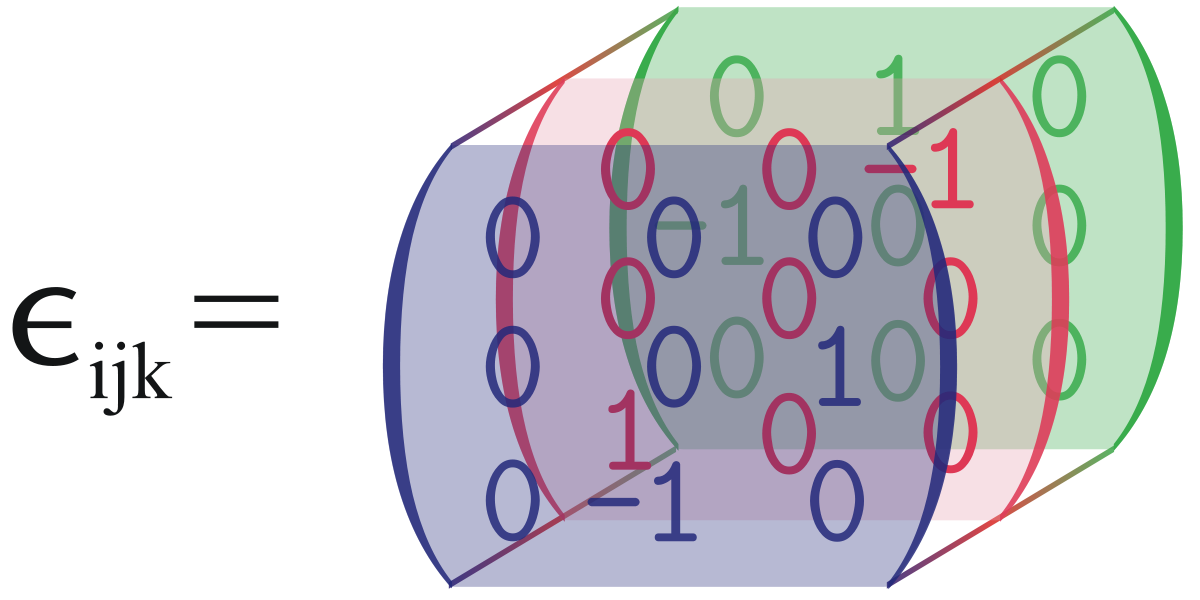
\includegraphics[scale=0.15]{levicivita.png}
\caption{Operador levi-civita representado como un tensor de orden 3}
\end{figure}

Ahora uno podría preguntarse para que sirve, como se aplica... Es irrelevante. Para nosotros no es más que un operador que nos permite escribir de manera reducida el producto vectorial. Lo introducimos porque me parece relevante conocer que estamos haciendo, ya que si uno piensa puede entender el porqué de esta relación (aún así hay que pensar bastante). Veamos primero como se formula la relación. Sean  dos vectores $A_i,B_i$ su producto vectorial se puede expresar como:

\begin{equation}
(\vec{A} \times \vec{B})_i = e_{ijk} A_j B_k
\end{equation}

Para pensarlo supongamos que vamos a calcular el primer término del producto vectorial. Si $i=1$, tenemos que los términos que van con 1 serán de $A_j$ y $B_k$ no estarán presentes en el valor, algo que desarrollaríamos de manera análoga si usaremos la fórmula del determinante. Entonces si tenemos que $j=2$ y $k=3$ lo que lo multiplica será positivo, y si $j=3$ y $k=2$ tenemos que lo que lo multiplica será negativo. Es decir:

$$ (\vec{A} \times \vec{B})_1 = A_2 B_3 - A_3 B_2 $$

lo cual ya sabíamos. Una vez tenemos este podemos imaginarnos el resto. Sean los vectores:

\begin{equation}
\begin{array}{ll}
\vec{A} = &  (t_{1 1}, t_{1 2}, t_{1 3}) \\
\vec{B} = &   (t_{2 1}, t_{2 2}, t_{2 3}) \\
\vec{C} = &  (t_{3 1}, t_{3 2}, t_{3 3})

\end{array}
\end{equation}

Podemos ver que también puede usarse para calcular determinantes, ya que:

\begin{equation}
\vec{A} \cdot (\vec{B} \times \vec{C}) = \epsilon_{ijk} A_i B_j C_k  = \begin{vmatrix}
t_{1 1} &
t_{1 2} &
t_{1 3} \\ 
t_{2 1} &
t_{2 2} &
t_{2 3} \\ 
t_{3 1} &
t_{3 2} &
t_{3 3} \\ 

\end{vmatrix} = |t_{ij}|
\end{equation}

Definimos como \textbf{pseudovectores} o \textbf{pseudotensores} a aquellos objetos que trasforman un escalar o un tensor pero cambiando el signo de la matriz de cambio por una de determinante -1. Es decir con trasformaciones impropias (véase \ref{Fig:3.1}). De hecho el símbolo de Levi-Civita como un pseudotensor de orden 3. \\

También son pseudvectores elementos como el momento angular o la velocidad angular. Esto es porque en su ley de transformación se introduce el símbolo de Levi-Civita, que como pseuodovector, lleva incorporada una trasformación impropia de tal manera que se acaba conviertiendo en un pseudovector. 

\section{Cinemática del cuerpo rígido}

Un cuerpo rígido es un sistema de partículas con posiciones relativas constantes. Para un sistema continuo esto significa que la distancia entre elementos de masa y masa diferencial de volumen permanecen constantes. En el límite de cotinuo a sólido:

\begin{equation}
\begin{array}{rll}
\mathrm{Masa \ total:}  &  M = \sum_i m_i  & \longrightarrow M = \int_V \D m  = \int_V \rho \D V \\ \\
\mathrm{Centro  \ de \ masas \ total:}  &   \vec{R_M} = \dfrac{1}{M} \sum_i m_i \vec{r_i}  & \longrightarrow \vec{R_M} = \dfrac{1}{M} \int_V \vec{r} \D m  \\  \\
\mathrm{Momento \ total:}  &  \vec{P} =  \sum_i m_i \vec{p_i}  & \longrightarrow \vec{R_M} = \dfrac{1}{M} \int_V \vec{p} \D m 
\end{array}
\end{equation}

Ahora solo tendremos que fijar un punto y la orientación de los tres ejes de coordenadas. \\

\subsection{Tensor de inercia:}

Sea un sistema discreto de partículas, la energía cinética viene dado por:

$$ T = \sum_{\alpha=1}^n \dfrac{1}{2} m_\alpha v_\alpha^2 $$
y la velocidad vendrá dada por:

\begin{equation}
\vec{v_\alpha} = \vec{v} + \vec{w} \times \vec{r_\alpha}
\end{equation}
donde $v$ es la velocidad de traslación y $w$ la de rotación. Si elevamos la velocidad al cuadrado va a aparecer un término que va con la velocidad de traslación, un término de velocidad angular y otro acoplado por ambos. El término acolado por ambos $\sum_i m_i v (w \times r_i)$ se anulará si el tomamos como origen del sistema el centro de masas. Esto es porque las velocidades $w \times r$ si no están al cuadrado se cancelarán una a una. Entonces tenemos que:

\begin{equation}
T = \dfrac{1}{2} M v^2 + \dfrac{1}{2} \sum_\alpha m_\alpha (\vec{w} \times \vec{r_\alpha})^2  = T_{tras} + T_{rot}
\end{equation}
llamando a este último término la energía de rotación, y que el módulo del producto vectorial puede reescribirse usando la siguiente fórmula:

\begin{equation}
(\vec{A} \times \vec{B})^2 = |A|^2|B|^2 \sin^2 \alpha  = |A|^2|B|^2 (1- \cos^2 \alpha) =  |A|^2|B|^2 - (A \cdot B)^2
\end{equation}
Por tanto podemos escribir la rotación como:

$$ \sum_\alpha (\vec{w} \times \vec{r}_\alpha)^2 = \sum_i \left[ w^2 r_\alpha^2 - (\vec{w} \cdot \vec{r_\alpha})^2 \right] = \sum_{\alpha} (\delta_{ij}   w_{i} w_{j} x_{\alpha,k} x_{\alpha,k} - x_{\alpha,i} x_{\alpha,j})  \Longrightarrow $$

\begin{equation} T_{rot} = \dfrac{1}{2} w_i \left[  \sum_{\alpha} m_\alpha (\delta x_{\alpha,k} x_{\alpha,k} -  x_{\alpha,i}  x_{\alpha,j} )    \right] w_j = \dfrac{1}{2} w_i I_{ij} w_j 
\end{equation}

Al tensor cuya ij componente se define de la siguiente manera se le llama \textbf{tensor de incercia}, y se entiende como una medida de cuanto cuesta hacer rotar a un cuerpo respecto a un eje de rotación, que vendrá dado por $\vec{w}$ con un determinado origen. Si cambiamos el origen y cambiamos el sistema de referencia (de ejes) el tensor de inercia variará. Sus componentes:

\begin{equation}
I_{ij}  =\sum_{\alpha}    m_\alpha (\delta x_{\alpha,k} x_{\alpha,k} -  x_{\alpha,i}  x_{\alpha,j} )   
\end{equation}


Podemos expresar la energía cinética de rotación como:

\begin{equation}
T_{rot} = \dfrac{1}{2} \vec{w} \cdot \mathbb{I} \cdot \vec{w} = \vec{2} \parentesis{ \sum_\alpha m_\alpha (\vec{r_\alpha}^2 \mathds{1} - \vec{r}_\alpha \otimes \vec{r}_\alpha )} \vec{w}
\end{equation}

Ahora, ¿Cual es el límite para un sólido rígido continuo? Para distribuciones continuas de materia:

\begin{equation}
\mathbb{I} = \int_V  \rho [\vec{r}^{ \ 2} \mathds{1} - \vec{r} \otimes \vec{r}] \D V
\end{equation}

El tensor de inercia es un tensor de segunda orden, tal y como ha quedado patente en su definición. Al ser un tensor se le pueden aplicar trasformaciones ortogonales igual que los vectores o los ejes. Además será real y simétrico, por lo tanto diagonalizable. Otra propiedad es que la suma de dos tensores de inercia que tienen el mismo punto de origen y sistema de referencia, pero de dos sistemas diferentes, si se suman se tendrá el mismo tensor que al calcular el tensor de ambos juntos. Es decir, son aditivos. Si la velocidad angular está dirigida en la dirección del eje de rotación, y $n$ es el vector unitario en esa dirección podemos calcular la energía de rotacion con un escalar

\begin{equation}
T = \dfrac{1}{2} I_n w^2
\end{equation}

donde $I_n$ será igual a:

\begin{equation}
I_n = \vec{n} \cdot \mathbb{I} \cdot \vec{n}
\end{equation}

Si diagonalizamos el momento de inercia obtendremos una serie de autovalores y una serie de autovectores. A estos autovectores los llamamos los ejes principales. Una manera rápida de encontrar los ejes de simetría de un objeto, ya que estos siempre van a ser ejes principales. Por ejemplo en una esfera, los tres ejes cartesianos son ejes de simetría, por lo que serán ejes principales. Una vez tenemos los ejes principales, tendremos que el tensor $\mathbb{I}$ será un tensor diagonal $$ \mathbb{I} = \begin{pmatrix}
I_{ 1 1 }  &
0  &
0 \\ 
0  &
I_{ 2 2 }  &
0 \\ 
0  &
0  &
I_{ 3 3 }  
\end{pmatrix} $$ y por lo tanto a cada eje podremos asignarle un momento de inercia. En función de estos momentos de inercia podremos clasificar los sólidos rígidos en.

\begin{itemize}
\item \textbf{Trompo esférico:} llamamos así a aquellos cuerpos en los que los momentos de los 3 ejes principales son iguales, es decir:  $I_{11} = I_{22} = I_{33}$ 
\item \textbf{Trompo simétrico:} llamamos así a aquellos cuerpos en los que los momentos de los 2 ejes principales son iguales, es decir:  $I_{11} = I_{22} \neq I_{33}$ (o cualquier otro sin pérdida de generalidad).
\item \textbf{Trompo asimétrico:} llamamos así a aquellos cuerpos en los que los momentos de los 3 ejes principales son diferentes, es decir:  $I_{11} \neq I_{22} \neq I_{33}$ 
\end{itemize}

\subsection{Momento angular}

Sabemos que el momento angular de un sistema de partículas respecto a un punto de referencia se puede definir como:

\begin{equation}
\vec{L} = \sum_{\alpha=1}^N  m_\alpha \vec{r}_\alpha \times \vec{v}_\alpha =\sum_{\alpha=1}^N  m_\alpha \vec{r}_\alpha \times  ( \vec{w}_\alpha \times \vec{r}_\alpha  )
\end{equation}
que si usamos la indentidad vectorial del vectorial del vectorial tenemos que:

\begin{equation}
\vec{L} = \sum_{\alpha = 1}^N m_\alpha [ \vec{r}_\alpha^2 \vec{w} - (\vec{r}_\alpha \cdot \vec{w}) \vec{r}_\alpha ]
\end{equation}
que es lo mismo que escribir componente a componente que:

\begin{equation}
L_{i} = \sum_{\alpha=1}^N ((x_{\alpha,k} x_{\alpha,k} ) w_j - x_{\alpha,i} x_{\alpha,j} w_j) = I_{ij} w_j
\end{equation}
lo que se puede escribir como:

\begin{equation}
\vec{L} = \mathbb{I} \cdot \vec{w}
\end{equation}

\subsection{Teorema de Steiner}

El teorema de Steiner nos relaciona el momento de inercia respecto a un punto concreto del plano con un sistema de rotación de ejes determinado, con el momento de inercia respecto a otro punto cualquiera. Si llamamos como $\vec{R}$ al vector que une el centro de masas del objeto y el nuevo origen sobre el que queremos calcular el momento de inercia, y a $X_i$ las componentes de este tenemos que cada componente del nuevo tensor de inercia vendrá dado por:

\begin{equation}
I_{ij} = I_{ij}^{CM} + M (\delta_{ij} R^2 + X_i X_j)
\end{equation}

Una versión reducida de este teorema nos da el momento de inercia respecto a un eje de inercia cualquiera a partir del momento de inercia del mismo eje pero que pasa por el centro de masas. Entonces si $d$ es la distancia entre ejes tenemos que:

\begin{equation}
I_n = I_n^{CM} + M d^2
\end{equation}

\section{Ecuaciones del movimiento}

En el caso de que no haya fuerzas externas sabemos que el movimiento del cuerpo será a velocidad constante o permanecerá en reposo, por lo que siempre podemos encontrar un sistema de referencia inercial donde no haya energía por traslación (resta de una constante arbitraria). Entonces la lagrangiana será la energía por rotación. Si diagonalizamos la matriz de rotación, es decir, si \textit{escribimos el momento de inercia respecto los ejes principales}:

\begin{equation}
T_{rot} = \frac{1}{2} I_{11} w_1^2 + \frac{1}{2} I_{22} w_2^2 + \frac{1}{2} I_{33} w_3^2 \label{Ec:3.5-051}
\end{equation}

Ahora para estudiar el problema del movimiento tenemos que estudiar las ecuaciones de Euler-Lagrange en función de los ángulos de rotación. Si usamos los ángulos de Euler que ya hemos introducido. Hagamos primero la del ángulo $\psi$:

\begin{equation}
\parciales{}{t} \pparciales{L}{\dot{\psi}} - \parciales{L}{\psi} =  \parciales{}{t} \pparciales{T}{\dot{\psi}} - \parciales{T}{\psi}  = 0
\end{equation}
si aplicamos la regla de la cadena par respecto $w_i$ obtenemos que:

\begin{equation}
\parciales{}{t} \parentesis{\parciales{T}{w_i} \parciales{w_i}{\dot{\psi}}} - \parciales{T}{w_i} \parciales{w_i}{\psi} = 0 
\end{equation}
y usando la ecuación \ref{Ec:3.1-017} y \ref{Ec:3.5-051} podemos llegar a que:

\begin{equation}
\parciales{w_1}{\psi} = \dot{\phi} \sin \theta \cos \psi - \dot{\theta} \sin \psi \tquad \parciales{w_2}{\psi} = - \dot{\phi} \sin \theta \sin \psi + \dot{\theta} \cos \psi \tquad \parciales{w_3}{\psi} = 0
\end{equation}

\begin{equation}
\parciales{w_1}{\dot{\psi}} = 0 \tquad \parciales{w_2}{\dot{\psi}} = 0 \tquad \parciales{w_3}{\dot{\psi}} = 1
\end{equation}
Ahora podremos obtener las ecuaciones del movimiento. La ecuación para los otros ángulos ($\theta,\phi$) es análoga, por lo que podemos obtener las siguientes ecuaciones del movimiento, las llamadas \textbf{ecuaciones de Euler}:

\begin{equation}
I_1 \dot{w_1} + (I_3 -I_2) w_2 w_3 = 0
\end{equation}
\begin{equation}
I_2 \dot{w_2} + (I_1 -I_3) w_2 w_3 = 0
\end{equation}
\begin{equation}
I_3 \dot{w_3} + (I_2 -I_1) w_2 w_3 = 0
\end{equation}
De forma vectorial (matricial):

\begin{equation}
\mathbb{I} \cdot \dfrac{\D \vec{w}}{\D t} + \vec{w} \times (\mathbb{I} \cdot \vec{w}) = 0 \Longrightarrow \dfrac{\D L}{\D t} + \vec{w} \times \vec{L} = 0
\end{equation}

O lo que es mejor, de manera tensorial:

\begin{equation}
I_i \dot{w_i} + \epsilon_{ijk} w_j (I_k w_k) = 0 \tquad (\mathrm{sin \ sumar \ los  \ i})
\end{equation}

\subsection{Caso con momentos generalizados}
Ahora vamos a estudiar el caso donde existen fuerzas generalizadas externas, que como estamos estudiando rotaciones, afectarán a la rotación de la partícula si son momentos (si no son momentos afectará al movimiento de traslación). En el caso de que haya fuerzas externas tendríamos que:

\begin{equation}
 \parciales{}{t} \pparciales{T}{\dot{\psi}} - \parciales{T}{\psi}  =  Q_{\psi}
\end{equation}
tal que la fuerza generalizada serán

\begin{equation}
Q_\psi = \vec{F} \cdot \parciales{\vec{r}}{\psi}; \tquad  Q_\phi = \vec{F} \cdot  \parciales{\vec{r}}{\phi}; \tquad Q_\theta = \vec{F} \cdot  \parciales{\vec{r}}{\theta}
\end{equation}
Tenemos además que $\D \vec{r} = \D \Omega \times \vec{r}$ implica que $$ \parciales{r_i}{\Omega_j} = \epsilon_{ikj} r_k $$. Entonces estudiemos el caso particular del ángulo $\psi$. Como las fuerzas generalizadas son productos escalares y estos se pueden expresar de forma tensorial:

\begin{equation}
Q_\psi = F_i \parciales{r_i}{\psi} = F_i \parciales{r_i}{\Omega_j} \parciales{\Omega_j}{\psi} 
\end{equation}
Dado que $\D \vec{\Omega} = \vec{w} \D t$ podemos usar la ecuación \ref{Ec:3.1-017} de tal manera que:

\begin{equation}
\parciales{\Omega_1}{\psi} = 
\parciales{\Omega_2}{\psi} = 0; \tquad 
\parciales{\Omega_3}{\psi} = 1
\end{equation}
Usamos esto para poder expresar la fuerza generalizada, de tal manera que:

\begin{equation}
Q_\psi = F_i \parciales{r_i}{\Omega_3} = F_i \epsilon_{i3k} r_k = (\vec{r} \times \vec{F})_3 = \vec{M}_3
\end{equation}
Eso nos lleva a deducir las nuevas ecuaciones del movimiento como:


\begin{equation}
I_1 \dot{w_1} + (I_3 -I_2) w_2 w_3 = M_1
\end{equation}
\begin{equation}
I_2 \dot{w_2} + (I_1 -I_3) w_2 w_3 = M_2
\end{equation}
\begin{equation}
I_3 \dot{w_3} + (I_2 -I_1) w_2 w_3 = M_3
\end{equation}
De forma vectorial (matricial):

\begin{equation}
\mathbb{I} \cdot \dfrac{\D \vec{w}}{\D t} + \vec{w} \times (\mathbb{I} \cdot \vec{w}) = \vec{M} \Longrightarrow \dfrac{\D L}{\D t} + \vec{w} \times \vec{L} = \vec{M} \label{Ec:3.5-068}
\end{equation}

De aquí podemos deducir que un cuerpo rígido libre no puede girar a $\vec{w}$ constante a no ser que lo haga alrededor de un eje principal, ya que si tanto $M$ commo $\D w/ \D t $ son ceros no queda otra que $w \times (\mathbb{I } \cdot w) = 0$ y esto conlleva a decir que $w$ y $\mathbb{I} \cdot w$ son paralelos. \\

Si multiplicamos la ecuación \ref{Ec:3.5-068} por $\vec{w}$ (producto escalar) tenemos que por ser $w$ perpendicular a $w \times (\mathbb{I} \cdot w)$ la ecuación queda de la siguiente manera:

\begin{equation}
\vec{w} \cdot \mathbb{I} \cdot \dfrac{\D \vec{w}}{\D t} = \vec{M} \cdot \vec{w}
\end{equation}

Es decir esto se puede escribir como:

\begin{equation}
\dfrac{1}{2} \dfrac{\D }{\D t} (\vec{w} \cdot \mathbb{I} \cdot \vec{w}) = \vec{M} \cdot \vec{w} \Longrightarrow \dfrac{\D}{\D t}T_{rot} = \vec{M} \cdot \vec{w}
\end{equation}

\chapter{Relatividad}

\section{Postulados y trasformaciones de Lorentz}

\subsection{Postulados}

Definimos \textbf{sistema de referencia inercial} como aquel sistema de referencia (sistema de coordenadas x,y,z y tiempo t) en el cual todas las leyes de la física se cumplen de manera habitual. También se define como cualquier sistema en el cual una partícula aislada, libre de interacciones o permanece en reposo o se mueve uniformemente.\\



Los dos postulados de la relatividad especial son:

\begin{itemize}
\item \textbf{Principio de relatividad:} las leyes de la Física son las mismas para cualquier momento inercial. Otra forma de mencionarla es que si un sistema $S$ es un sistema inercial si un segundo sistema $S'$ se mueve con velocidad constante relativa a $S$, entonces $S'$ también es un sistema inercial.

\item \textbf{Principio de constancia de la velocidad de la luz:} la velocidad de la luz en el vacío es una constante universal, independientemente de cualquier movimiento de la fuente u observador.
\end{itemize}


\subsection{Trasformaciones de Galileo}

Las trasformaciones de Galileo son las trasformaciones que rigen al mundo clásico,, ya que considera el tiempo un valor absoluto, igual para todos los sistemas de referencia.  Sean las coordenadas sin primar aquellas del sistema inercial que está quieto, y el primado el que se mueve respecto este, y $u$ su velocidad. Si consideramos una trasformación unidimensional (suponemos que no se mueve a lo largo de las coordenadas $x'_2$ y $x'_3$) tenemos que:

\begin{equation}
\begin{array}{rcl}
x_1'&  = & x_1 - ut \\
x_2' & = & x_2 \\
x_3' & = & x_3 \\
t' & = &  t
\end{array}
\end{equation}

En este caso para un rayo de luz emitido en $t=0$ y origen de los sistemas (no es postulado que la velocidad de la luz se conserve, solo el tiempo es absoluto). Nombrando a $x_1 \equiv x$ y $x_1' \equiv x'$:

$$ x' = c't' = c' t ; \quad x = c t \Longrightarrow x - ut = c' t \Longrightarrow c - u = c' $$


\subsection{Trasformaciones de Lorentz}
Las trasformaciones de Lorentz modifican la manera que entendemos el mundo. Estudiaremos sus consecuencias en el siguiente punto. Agrupando, las \textbf{trasfromaciones de Lorentz} para el caso unidimensional:

\begin{equation}
\begin{array}{rll}
t' & = & \gamma \parentesis{ t - \dfrac{v}{c^2} x_1} \\ \\

x_1' & = & \gamma \parentesis{x_1 - vt} \\ \\

x_2 ' &  = & x_2 \\ \\

x_3 ' & = & x_3
\end{array} \label{Ec:4.1.2-002}
\end{equation}

Donde llamamos al \textbf{factor gamma} o \textbf{factor de Lorentz} a:

\begin{equation}
\gamma = \sqrt{\dfrac{1}{1 - \beta^2}}  \tquad \beta = \dfrac{v}{c}
\end{equation}

Antes de continuar vamos a definir varios conceptos que nos serán útiles al estudiar las consecuencias de la relatividad especial. Llamamos a dos sucesos que ocurren en el mismo instante \textit{simultáneos}, y dos sucesos que ocurren en el mismo lugar \textit{colocales}. Dos sucesos simultáneos y colocales son \textit{coincidentes}. Supongamos los sucesos A y B. Como las trasformaciones son lineales, tenemos que las diferencias de espacio y tiempo que ocurren entre dos sucesos se trasforman igual que las coordenadas:

\begin{equation}
\begin{array}{rll}
\Delta t' & = & \gamma \parentesis{  \Delta t - \dfrac{v}{c^2}  \Delta x} \\ \\
\Delta x' & = & \gamma \parentesis{\Delta x - v\Delta t}
\end{array} 
\end{equation}
Cambiando:

\begin{equation}
\begin{array}{rll}
\Delta t & = & \gamma \parentesis{  \Delta t' + \dfrac{v}{c^2}  \Delta x'} \\ \\
\Delta x & = & \gamma \parentesis{\Delta x' + v\Delta t'}
\end{array} 
\end{equation}

  Las transformaciones de Lorentz son lineales (con un factor gamma que sería el ``factor de proporcionalidad''). De hecho se puede demostrar que las transformaciones \textit{han} de ser lineales, ya que si no no se podría conservar la calidad de inercial de un sistema ante la transformación de Lorentz: si el movimiento uniforme en un sistema ha de transformarse en otro movimiento uniforme en otro sistema la transformación debe ser lineal. \\
  

Como podemos ver las transformaciones de Lorentz verifican completamente las condiciones que impusimos: que la velocidad de la luz sea constante y que las leyes de la física (en espacial las de Maxwell) sean correctas y válidas en todo sistema de referencia inercial. Ahora supongamos que de un punto del espacio se envía una onda de luz.  El frente de ondas en un tiempo $t$ se encontrará a :

\begin{equation}
x^2 + y^2 + z^2  = c^2 t^2
\end{equation}

Si aplicamos las transformaciones de Lorentz que el frente de ondas que se observa para un sistema primado (en movimiento) es esférico y se propaga con velocidad $c$. Entonces:

\begin{equation}
x'^2 + y'^2 + z'^2 = c^2 t'^2
\end{equation}

Como hemos mencionado la teoría de la relatividad especial de Einstein es una teoría de la relatividad, por lo que es de esperar que las ecuaciones de transformación de Lorentz sean verdaderamente relativas: la transformación inversa tenga la misma forma con $v$ pero cambiada de signo:


\begin{equation}
\begin{array}{rll}
t & = & \gamma \parentesis{ t' + \dfrac{v}{c^2} x_1'} \\ \\

x_1 & = & \gamma \parentesis{x_1 ' + vt'} \\ \\

x_2  &  = & x_2 ' \\ \\

x_3  & = & x_3'
\end{array}\label{Ec:4.1.2-008}
\end{equation}


\subsection{Dilatación temporal}

Supongamos que dos sucesos son coincidentes en el espacio de referencia $S'$, tal que $\Delta ' = 0$ y $\Delta t' \neq 0$. En el espacio de referencia $S$ estos sucesos \textit{no} serán colocales, por lo que si despejamos obtenemos que:

$$ \Delta t' = \dfrac{\Delta t}{\gamma}$$

Es decir obtenemos que el tiempo trascurrido entre ambos sucesos será menor para el sistema de referencia $S'$ que para el sistema de referencia $S$. Es mucho mas sencillo de ver para un ejemplo. \\

Supongamos que estamos en un tren en movimiento, y nos quedamos dormidos, siendo este el suceso $A$, despertándonos en la siguiente estación (suceso $B$). Para nosotros, este suceso es colocal: nos dormimos y nos despertamos en el mismo asiento. Obviamente para alguien que este en una de las estaciones no, tu te dormirás en la primera estación pero te despertarás en la segunda: no es la misma posición. En el caso relativista será similar: obviamente los dos sucesos para quien está en la estación no es colocal. En el caso de las trasformaciones relativistas entre ambos sucesos no habrá la misma diferencia temporal, es decir, para la persona que se durmió entre ambos sucesos habrá ocurrido un tiempo $\Delta t'$ que será diferente (menor) que para la persona de la estación, ya que:

\begin{equation}
\Delta t = \gamma \Delta t'
\end{equation}

El tiempo que trascurre entre dos sucesos en un sistema de referencia que los hace colocales se llama \textbf{tiempo propio}, y para cualquier otro sistema de referencia el tiempo será mayor. A esta relación se le llama \textbf{dilatación temporal}.

\subsection{Contracción de longitudes}

Supongamos una barra que su longitud de reposo es $L_0 = \Delta x$, sin que $\Delta t = 0$, ya que para cualquier momento ambos puntos se encontrarán a la misma distancia. Ahora para un observador en movimiento su longitud será $L = \Delta x'$. Medimos los extremos de la barra en el mismo instante $\Delta t' = 0$ (ya que no medirá lo mismo). 

\begin{equation}
L_0 = \gamma L \longleftrightarrow L = \dfrac{L_0}{\gamma}
\end{equation}

es decir un observador en movimiento mide siempre una longitud menor que su longitud en reposo. A este fenómeno se llama \textit{contracción de longitudes}. 

\subsection{Trasformación de velocidades}

Tenemos que por definición:

\begin{equation}
\begin{array}{lll}
v_x & = & \dfrac{\D x}{\D t} \\ \\
v_x' & = & \dfrac{\D x'}{\D t'}
\end{array}
\label{Ec:4.1.6-012}
\end{equation}

Las transformaciones de Lorentz de manera infinitesimal:


\begin{equation}
\begin{array}{lll}
\D x' = \gamma (\D x - v \D t) & \tquad & \D t' = \gamma (\D t - \frac{v}{c^2} \D x) \\ \\
\D x = \gamma (\D x' + v \D t') & \tquad & \D t = \gamma (\D t' + \frac{v}{c^2} \D x') \\
\end{array} 
\end{equation}

Podemos substituir en la ecuación \ref{Ec:4.1.6-012} los valores infenitesimales obteniendo unas velocidades en función de otras:

$$
v_x = \dfrac{\gamma (\D x' + \beta c \D t'}{\gamma (\D t' + (\beta/c) \D x'))} = \dfrac{\frac{\D x'}{\D t'} + v }{1+\frac{v}{c^2} \frac{\D x'}{\D t}}
$$

O lo que es lo mismo:

\begin{equation}
v_x = \dfrac{v_x'+v }{1 + \frac{v}{c^2} v_x'}
\end{equation}

Es decir que para un sistema de referencia la velocidad de un objeto será diferente de la velocidad del mismo objeto en otro sistema de referencia. A esta relación se le conoce como \textit{regla relativista de adicción de velocidades}. \\

Si consideramos las otras coordenadas $x_2$ y $x_3$ tenemos que las velocidades en estas también se trasforman ya que $\D t$ no depende solo de $\D t'$, aunque el objeto no se mueva en estas coordenadas:


\begin{equation}
v_y = \dfrac{v_y'}{\gamma(1 + \frac{v_x' v}{c^2})}
\end{equation}
\begin{equation}
v_z =  \dfrac{v_z'}{\gamma(1 + \frac{v_x' v}{c^2})}
\end{equation}




\section{Formalismo cuadrimensional}



Las transformaciones de Lorentz nos revelan como son los cambios de coordenadas entre sistemas de coordenadas que se muevan uniformemente uno respecto a otro. Tiene la forma de una transformación lineal de un sistema de cuatro coordenadas a otro coordenadas. Si designáramos la coordenada cero de un espacio cartesiano a la coordenada $i ct$ tenemos que el producto escalar del vector de posición en el cuadriespacio será:

\begin{equation}
x_0^2 + x_1^2 + x_2^2 + x_3^2 = -c^2 t^2 + x^2 + y^2 + z^2 
\label{Ec:4.2.0-016}
\end{equation}

que en virtud de las ecuaciones del frente de ondas tenemos que el producto de dicho espacio será invariante frente a una transformación de ondas. A este cuadriespacio que no varía frente a una transformación de Lorentz se le llama \textit{espacio de Minkowski}. Así pues \textit{la transformación de Lorentz es una transformación ortogonal en el espacio de Minkowski}.\\


% leer pagina 356 goldstein para ver mas interesante cosas super mega hiper chulis sobre relatividad especial

Aunque sea interesante que podamos crear un espacio cuadrimensional con la primera coordenada compleja de tal forma que el espacio de Minkowski sea cartesiano, y que la transformada de Lorentz es compleja, podemos crear un espacio donde esta este definida en un espacio real. En dicho espacio podemos crera una coordenada $x_0 = ct$ de tal forma $t = x_0/c; t' = x_0'/c$. Sin embargo de ser así el espacio real no puede ser euclídeo, sino que se denomina espacio de \textit{Rimenan}, con un tensor métrico diagonal $G$ (el tensor métrico es aquel que mide el espacio en una dimensión) que tiene que ser:


\begin{equation}
G = \begin{pmatrix}
-1 &
0 & 
0 & 
0 \\
0 & 
1 &
0 & 
0 \\ 
0 &
0 & 
1 &
0 \\ 
0 & 
0 & 
0 & 
1 
\end{pmatrix}
\end{equation}

Ahora bien, ¿Se verificará que el producto escalar es como en la ecuación \ref{Ec:4.2.0-016}? Como el producto escalar en un espacio méctrico cualquiera viene dado por:

\begin{equation}
x \cdot G \cdot x^T = - x_0^2 + x_1^2 + x_2^2 + x_3^2
\end{equation}

por lo que se verifica, siendo este un \textbf{espacio de Minkowski}. Según las ecuaciones de la transformación de Lorentz \ref{Ec:4.1.2-002} y \ref{Ec:4.1.2-008} podremos escribir la matriz de cambio de coordenadas relativista como:



\begin{equation}
\Lambda = 
\begin{pmatrix}
\gamma &
- \beta \gamma &
0 & 0 \\ 
- \beta \gamma &
\gamma &
0 & 0\\ 
0  &
0  &
1 & 0 \\
0 & 0 & 0 & 1
\end{pmatrix}
\end{equation}

tal que el cambio de coordenadas será:

\begin{equation}
\begin{pmatrix}
x^{0'}\\ 
x^{1'}\\ 
x^{2'}\\ 
x^{3'}
\end{pmatrix} = 
\begin{pmatrix}
\gamma &
- \beta \gamma &
0 & 0 \\ 
- \beta \gamma &
\gamma &
0 & 0\\ 
0  &
0  &
\gamma & 0 \\
0 & 0 & 0 & \gamma
\end{pmatrix}
\begin{pmatrix}
x^{0} \\ 
x^{1} \\ 
x^{2} \\ 
x^{3} 
\end{pmatrix}
\end{equation}




 Entonces las trasformaciones de Lorentz son trasformaciones lineales en un espacio de 4 dimensiones del cuales sus elementos son vectores de cuatro componentes: los \textbf{cuadrivectores}.

\begin{equation}
\mathbb{X} = (x^0, x^1, x^2, x^3)
\end{equation}

pudiendo escribir
\begin{equation}
\mathbb{X}' = \Lambda \cdot \mathbb{X}
\end{equation}

Decimos que los escalares de cuadrivectores en el espacio de Minkowski son invariantes Lorentz. Podemos definir asi cualquier escalar (masa, energía...) vectores (velocidad, posición, momento...) y tensores de segundo orden (tensor de Maxwell...), ya que el principio de relatividad afirma que todas las leyes de la física deben ser válidas tras una transformación de Lorentz, lo cual se verifica ya que los tensores:

\begin{equation}
\mathbb{A} = \mathbb{B} \Longrightarrow \mathbb{A}' = \mathbb{B}'
\end{equation}

ya que ambos miembros se transforman de la misma manera (lo que llamamos \textit{transformacón covariante}). 

\subsection{Intervalos}

Un suceso o acontecimiento es un vector en el espacio de Minkoswki. Si designamos un suceso (un vector posición de 3 coordenadas espaciales y un tiempo) como $\mathbb{X}_A$ y otro como $\mathbb{X}_B$ definimos como \textbf{intervalo} de dos sucesos como:

\begin{equation}
S_{AB}^2 = (\mathbb{X}_B - \mathbb{X}_A)^2 = (\Delta X)^2 
\end{equation}

que por ser el producto escalar podemos hacerlo suponiendo la coordenada temporal compleja o usando la métrica de Riemann. Cualquiera de los dos es válido, y se obtiene que:

\begin{equation}
S_{AB}^2 = -c^2 \Delta t^2 + (\Delta \vec{r})^2 
\end{equation}

donde $(\Delta \vec{r})^2 $ designado a veces como $d_{AB}^2$ es la distancia euclídea entre ambas posiciones espaciales, y $\Delta t$ el intervalo temporal entre ellos. En función de como se encuentren en el espacio de minkowski las posiciones tenemos que el intervalo puede ser negativo, positivo o nulo. En función de esto diferenciamos los siguientes intervalos:

\begin{itemize}
\item \textbf{Intervalo tipo espacio:} en este caso $S_{AB}^2 > 0$ por lo que la distancia es mayor que $c \Delta t$.  Entonces los sucesos están separados por una distancia mayor que la que recorre la velocidad de la luz en un tiempo $\Delta t$. Otra forma de verlo es que \textit{un rayo de luz no le da tiempo a conectar ambos sucesos}. Un ejemplo claro es aquel donde los sucesos son simultáneos en posiciones distintas.
\item \textbf{Intervalo tipo luz:}  $ S_{AB} = 0 $. Los sucesos están separados por una distancia exactamente igual a la recorre la velocidad de la luz en un tiempo $\Delta t$. 
\item \textbf{Intervalo tipo tiempo:} $S_{AB} < 0$. Los sucesos están separados por una distancia mas pequeña que la que recorre la velocidad de la luz en el intervalo temporal. El caso mas claro son los sucesos colocales en instantes diferentes.
\end{itemize}
 
En función de si los sucesos son de tipo espacio, luz o tiempo nos permite deducir si los sucesos pueden ser coincidentes, colocales o simultáneos en algún sistema de referencia. Por ejemplo si dos sucesos tienen un intervalo de tipo espacio, tenemos que estos nunca van a poder ser colocales para ningún tipo de sistema de referencia, pero van a poder ser simultáneos. Para dos sucesos de intervalo de tipo tiempo es imposible encontrar un sistema en el que sean simultáneos, pero si que sean colocales. 

\subsection{Cono de luz}

Esto se puede estudiar gráficamente de manera muy sencilla usando os \textit{conos de luz}.


\section{Mecánica relativista}

\subsection{Tiempo propio}

Sabemos que que los postulados de la relatividad implican que las relaciones como el tiempo, el espacio... implican transformaciones Lorentz. Algunas de ellas tal y como el producto escalar de los cuadrivectores definidos en el espacio de Minkowski (lo que viene siendo el intervalo entre dos sucesos) son invariantes. Entonces podemos crear un \textbf{intervalo infenitesimal} de sucesos que sea invariante Lorentz tal que:

\begin{equation}
\D s = \sqrt{G_{\mu \nu} \D x^{\mu} \D x^{\nu}} = \sqrt{- c^2 \D t^2 + \D \mathbf{r}^2}
\end{equation}

Evidentemente tendrá coordenadas de distancia, y podemos hacerla temporal si dividimos entre $c^2$, tal que:

\begin{equation}
\D \tau^2 = - \dfrac{\D s^2}{c^2} = \D t^2 - \dfrac{1}{c^2} \D \mathbf{r}^2 \label{Ec:4.3.1-028}
\end{equation}

será un invariante Loretnz, pero con dimensiones temporales. A esta cantidad infinitesimal se le llama \textit{tiempo propio} y es el invariante que usaremos cuando tratemos de definir los cuadrivectores velocidad y aceleración. Sacamos factor común $\D t$ tenemos que:

\begin{equation}
\D \tau = \D t \sqrt{1+\dfrac{1}{c} \dfrac{\D \mathbf{r}^2}{\D t^2}} 
\end{equation}

de lo que se deduce que:

\begin{equation}
\D \tau = \dfrac{\D t}{\gamma}
\end{equation}



\subsection{Velocidad y aceleración}

Podemos definir un \textit{cuadrivector velocidad} $\mathbb{V}$. Este cuadrivector no será mas que la derivada entre el cuadrivector y el tiempo propio definido en \ref{Ec:4.3.1-028}, tal que:

\begin{equation}
v^{\mu} = \dfrac{\D x^{\mu}}{\D\tau}
\end{equation}


\begin{equation}
\mathbb{V} = (v^0, \mathbf{v}_{rel}) = \gamma \dfrac{\D}{\D t} (ct,\mathbf{r}) = \gamma \left( c, \dfrac{\D \mathbf{r}}{\D t} \right) = \gamma (c, \mathbf{v})
\end{equation}

donde el cuadrado del cuadrivector será un invariante:

\begin{equation}
\mathbb{V}^2 = G_{\mu,\nu} v^{\mu} v^{\nu} = v_\mu v^\mu = \gamma^2(-c^2 + \mathbf{v}^2) = - c^2
\end{equation}

ya que la velocidad de la luz es constante para cualquier sistema de referencia. También podemos definir un \textit{cuadrivector aceleración}.

\subsection{Momento}

En la mecánica relativista definimos como \textbf{cuadrivector momento}, tal que:

\begin{equation}
p^{\mu} = m v^{\mu}
\end{equation}

donde $m$ es un invariante con dimensión de masa. Tenemos pues que:

\begin{equation}
\mathbb{P} = (p^0, \mathbf{p}_{rel}) = m \gamma (c, \mathbf{v})
\end{equation}

\begin{equation}
\mathbb{P}^2 = m^2 (v) \mathbb{V}^2 =  - m^2 (v) c^2
\end{equation}

Donde podemos definir la cantidad $m(v) = m \gamma$ un parámetro llamado muchas veces \textbf{masa relativista}; siendo $m(v=0) = m$ la \textit{masa en reposo}, que es un invariante Lorentz. \\ 

La componente temporal del cuadrimomento es equivalente a $p^0 = \frac{E}{c}$ definida la energía como $E = m \gamma c^2$. Con esta definición de momento se puede ver que la conservación del momento es compatible con las transformaciones de Lorentz. Eso conlleva a que:

\begin{equation}
\sum \mathbb{P}_{inicial} = \sum \mathbb{P}_{final}
\end{equation}

Las componentes espaciales de la expresión dan la conservación del trimomento relativista y las coordenadas temporales dan otra ley de conservación que identificamos con la energía.

\subsection{Fuerza y energía}

El cuadrivector fuerza es tal que:

\begin{equation}
F^\mu = \dfrac{\D p^\mu}{\D \tau}
\end{equation}

\begin{equation}
\mathbb{F} = (F^0, \mathbf{F}_{rel}) = \dfrac{\D}{\D \tau} \mathbb{P} = \gamma \dfrac{\D }{\D t} (m \gamma c, m \gamma \mathbf{v}) 
\end{equation}

Donde podemos identificar las coordenadas espaciales y las coordenadas temporales. Las ecuaciones del movimiento serían las coordenadas espaciales. Podemos definir el trabajo tal que:

\begin{equation}
W_{12} = \int_1^2 \mathbf{F} \D \mathbf{r}
\end{equation}

o lo que es lo mismo:

\begin{equation}
W_{12} = T = \int_1^2 \dfrac{\D }{\D t} (m  \gamma \mathbf{v}) \cdot \mathbf{v} \D f = m \int_0^{v} \mathbf{v} \cdot \D (\gamma \mathbf{v}) 
\end{equation}

que si integramos por partes:

$$ T = m \gamma  \mathbf{v}^2 - m \int_0^v \gamma \mathbf{v} \D \mathbf{v} =  m \gamma  \mathbf{v}^2  - m \int \dfrac{\frac{1}{2} \D v^2}{\sqrt{1- \frac{v^2}{c^2}}} =  m \gamma  v^2  + m c^2 \left[   \sqrt{1-\frac{v^2}{c^2}} v^2 \right]^v_0  $$ 
$$
T = m \gamma v^2 + \dfrac{m}{\gamma} c^2- m c^2  =  m \gamma c^2 - m c^2
$$

Es decir la expresión relativista para la energía cinética es:

\begin{equation}
T = m \gamma c^2 - mc^2
\end{equation}

Si definimos energía total como $E = m \gamma c^2$ tenemos que:

\begin{equation}
E = T + mc^2 = t + E_0
\end{equation}

donde $E_0$ es la \textit{energía en reposo}, recuperando así la conservación de la masa-energía. Si nos vamos a la expresión del cuadrimomento podemos ver que su componente temporal ahora es:

\begin{equation}
\mathbb{P} = \parentesis{\frac{E}{c}, \mathbf{p}}
\end{equation}

por lo que momento y energía están ligados, tal y como lo están el espacio tiempo (ya que forman parte del mismo cuadrivector). Ahora la conservación de la energía y momento no son cosas separadas: solo existe la conservación del cuadrimomento, ya que $\mathbb{P}$ es un invariante Lorentz, tal que:

\begin{equation}
\mathbb{P}^2 = -m^2 c^2 = - \dfrac{E^2}{c^2} + p^2 
\end{equation}

donde podemos obtener la \textit{relación de dispersión}:

\begin{equation}
E^2 = p^2 c^2 + m^2 c^4
\end{equation}


\end{document}

